\documentclass[dvipdfmx,a4j]{jsarticle}
\setlength {\textwidth} {46zw} %横43文字
\setlength {\textheight} {46\baselineskip} %縦46行
\setlength{\topmargin}{-2.5cm} %2.5cm詰める

% パッケージと呼ばれるオプションをつける.
\usepackage{color} %色のオプション
\usepackage{listings}
\usepackage{amsmath}
\usepackage{ascmac}
\usepackage{amsmath,amssymb}
\usepackage{enumerate}
\usepackage{tikz}
\usepackage{graphicx}
\usepackage{here}
\usepackage{bm}

% ソースコードを貼る詳細設定
\lstset{
	%プログラム言語(複数の言語に対応,C,C++も可)
 	language = Python,
 	%枠外に行った時の自動改行
 	breaklines = true,
 	%自動開業後のインデント量(デフォルトでは20[pt])	
 	breakindent = 11pt,
 	%標準の書体
 	basicstyle = \ttfamily\small,
 	%basicstyle = {\small}
 	%コメントの書体
	 commentstyle = {\itshape \color[cmyk]{1,0.4,1,0}},
 	%関数名等の色の設定
 	classoffset = 0,
 	%キーワード(int, ifなど)の書体
 	keywordstyle = {\bfseries \color[cmyk]{0,0.8,1,0}},
 	%""で囲まれたなどの"文字"の書体
 	stringstyle = {\ttfamily \color[rgb]{0,0,1}},
 	%枠 "t"は上に線を記載, "T"は上に二重線を記載
	%他オプション:leftline,topline,bottomline,lines,single,shadowbox
	frame={TB},
 	%frameまでの間隔(行番号とプログラムの間)
 	framesep = 5pt,
 	%行番号の位置
 	numbers = left,
	%行番号の間隔
 	stepnumber = 1,
	%右マージン
 	%xrightmargin=0zw,
 	%左マージン
	%xleftmargin=3zw,
	%行番号の書体
 	numberstyle = \tiny,
	%タブの大きさ
 	tabsize = 4,
 	%キャプションの場所("tb"ならば上下両方に記載)
 	captionpos = t
}

\title{最適化と認識・学習}
\author{}

\begin{document}
\maketitle 
\section{導入}
最適化とは
\begin{eqnarray*}
  \Psi (\theta)\ &:&\ 目的関数\\
  \theta\ &:&\ パラメータ
\end{eqnarray*}
としたとき, $\Psi(\theta)$を$\theta$で最小化(あるいは最大化)することである.\ つまり\\
\centerline{\textcolor{red}{\large 関数の最小値, 最大値を与える$x$をもとめる問題}}\\
ということである.
\begin{center}
  \begin{tikzpicture}[>=stealth]
    \draw[->] (-0.7,0)--(4.5,0) node[right] {$x$};
    \draw[->] (0,-0.3)--(0,4.5) node[above] {$y$};
    \draw [domain=-0.3:3.4] plot(\x,{0.5*\x*\x-\x+1.5});
    \draw[draw=red,->,thick] (1,0)--(1,1);
    \draw[dashed] (1,0)--(1,0) node[below] {$x_{0}$};
    \draw[dashed] (1,1)--(0,1) node[left] {$f_{0}$};
    \node at (-0.5,2.2) {$f(x)$};
  \end{tikzpicture}
\end{center}
  このときの
\begin{eqnarray*}
    f_{0}&=&\underset{x}{\rm min}\,f(x)\\
    x_{0}&=&\underset{x}{\rm argmin}\,f(x)
\end{eqnarray*}
を求める問題である.
$\theta$が関数の形状を決めるパラメータであったとき, 目的関数$\Psi(\theta)$は近似誤差を表す関数となり, 最適化は関数$f(x;\theta)$の形状を求める問題といえる.

\section{回帰/分類とニュートン法, 勾配法}
勾配法は近似解を与え, 近似解の周辺の傾き等を用いて, 近似解を漸次改良し, この処理をくり返す方法である.\\
(例)\ 最急降下法, 共役勾配法, ニュートン法\\
\begin{center}
    \begin{tikzpicture}[>=stealth]
        \draw[fill=gray!20,rotate=50,xscale=1.9] (1.5,2) circle[radius=2];
        \draw[fill=gray!30,rotate=50,xscale=1.9] (1.7,2) circle[radius=1.7];
        \draw[fill=gray!40,rotate=50,xscale=1.9] (1.8,2) circle[radius=1.5];
        \draw[fill=gray!60,rotate=50,xscale=2] (1.8,2) circle[radius=1.3];
        \draw[fill=gray!70,rotate=51,xscale=2] (2,1.9) circle[radius=1];
        \draw[fill=magenta,draw=black] (-2,2) circle[radius=0.1];
        \draw(-2.1,2)--(-2.1,2) node[left]{$\mbox{\boldmath $x$}_{0}$};
        \draw[->,draw=green,very thick] (-1.9,2)--(-1.1,2);
        \node at(-1.5,1.7) {$-\nabla f(\mbox{\boldmath $x$}_{0})$};
        \node at(-1.5,1.35) {$H(\mbox{\boldmath $x$}_{0})$};
        \draw[->,draw=blue] (-1.9,2.05)--(-0.6,2.45);
        \draw[fill=magenta,draw=black] (-0.5,2.5) circle[radius=0.1];
        \draw(-0.5,2.4)--(-0.5,2.4) node[below] {$\mbox{\boldmath $x$}_{1}$};
        \draw[->,draw=green,very thick] (-0.42,2.55)--(0.32,3.55);
        \draw[->,draw=blue] (-0.42,2.55)--(1.03,3.93);
        \node at(0.8,3) {$-\nabla f(\mbox{\boldmath $x$}_{1})$};
        \node at(0.8,2.65) {$H(\mbox{\boldmath $x$}_{1})$};
        \draw[fill=magenta,draw=black] (1.1,4) circle[radius=0.1];
        \draw (1.1,4.05)--(1.1,4.05) node[above left] {$\mbox{\boldmath $x$}_{2}$};
        \draw[->,draw=green,very thick] (1.15,4.1)--(1.49,4.86);
        \draw[->,draw=blue] (1.15,4.1)--(1.84,5.17);
        \node at(2.2,4.6) {$-\nabla f(\mbox{\boldmath $x$}_{2})$};
        \node at(2.2,4.25) {$H(\mbox{\boldmath $x$}_{2})$};
        \draw[fill=red] (1.9,5.3) circle[radius=0.15];
        \node at(-2.3,3) {適当な初期値};
    \end{tikzpicture}
\end{center}
このように近似解を繰り返し修正することで最適値へ近づいていく. 勾配(, ヘシアン), つまり$E$の$\mbox{\boldmath $x$}_{0}$における1次(,2次)の微分)施すことで修正を行う. \\
問題としては近似解の精度を上げるために\textcolor{red}{どちらの方向にどれだけ}動かすか?ということである.
\subsubsection{最急降下法}
最急降下法は最も単純なもので勾配の方向に適当量移動させるという方法である. 式にすると以下のように表すことができる.
\begin{align*}
    x_{i+1}=x_{i}-\alpha \nabla f(\mbox{\boldmath $x$}_{i}) \tag{3.4}
\end{align*}
イメージ図としては以下のようになる.
\begin{center}
    \begin{tikzpicture}[>=stealth]
        \draw[rotate=40,fill=gray!16,xscale=2] circle[radius=2.1];
        \draw[rotate=40,fill=gray!20,xscale=2] circle[radius=1.9];
        \draw[rotate=40,fill=gray!30,xscale=2] circle[radius=1.7];
        \draw[rotate=40,fill=gray!35,xscale=2] circle[radius=1.5];
        \draw[rotate=40,fill=gray!40,xscale=2] circle[radius=1.2];
        \draw[rotate=40,fill=gray!50,xscale=2] circle[radius=0.7];
        \draw[rotate=40,fill=gray!80,xscale=2] circle[radius=0.3];
        \draw[rotate=40,fill=gray,xscale=2] circle[radius=0.05];
        \draw[fill=magenta] (-3,-1.4) circle[radius=0.1];
        \draw[->,very thick,draw=blue] (-2.93,-1.45)--(-2,-2);
        \draw[->,very thick,draw=blue] (-2,-2)--(-0.6,-0.6);
        \node at(-3.2,-2) {$-\nabla f(\mbox{\boldmath $x$}_{0})$};
        \node at(-3.7,-1.4) {$\mbox{\boldmath $x$}_{0}$};
    \end{tikzpicture}
\end{center}
誤差が最小となるところに持っていく. ということは誤差関数において値が最小となるように持ってくることである. つまり誤差関数の現時点にいる場所から傾きを得る. それが負であれば$+$にずらし, 正なら$-$にずらすことで最小値に近づけることが可能となる. 誤差関数が二次関数においての例は以下である.
\begin{center}
    \begin{tikzpicture}[>=stealth]
    \draw[very thick,domain=-3:3] plot(\x,{\x*\x/2});
    \draw[->] (-3,0)--(3,0) node[right] {$x$};
    \draw[->] (0,-0.3)--(0,5) node[above] {$y$};
    \node at(-0.2,-0.2) {O};
    \draw[thick,domain=1.5:2.5,draw=red] plot(\x,{2*\x-2});
    \draw[fill=magenta] (2,2) circle[radius=0.08];
    \draw[fill=magenta] (-2,2) circle[radius=0.08];
    \node at(4.3,2) {傾きが$+$なので$-$方向へ};
    \draw[thick,domain=-2.5:-1.5,draw=red] plot(\x,{-2*\x-2});
    \node at(-4.3,2) {傾きが$-$なので$+$方向へ};
    \end{tikzpicture}
\end{center}
最急降下法のアルゴリズムは以下のように表すことができる.\\[0.1cm]
$i_{0},\ x_{0}$を決める.\\
収束するまで繰り返し\{\\
\hspace{1cm} $x_{i+1}=x_{i}-\alpha \nabla f(\mbox{\boldmath $x$}_{i})$\\
\hspace{1cm} $i=i+1$\\
\}\\[0.1cm]
$\alpha$の決め方は様々であり, $-\nabla f(\mbox{\boldmath $x$})$の最適値を解析的に求めるかラインサーチによって求めて移動する. このときの移動量は同じであるが過去の勾配の大きさの履歴に応じて移動量を決定する.
\begin{center}
    \begin{tikzpicture}[scale=1.2,>=stealth]
        \draw[rotate=40,fill=gray!16,xscale=2] circle[radius=2.1];
        \draw[rotate=40,fill=gray!20,xscale=2] circle[radius=1.9];
        \draw[rotate=40,fill=gray!30,xscale=2] circle[radius=1.7];
        \draw[rotate=40,fill=gray!35,xscale=2] circle[radius=1.5];
        \draw[rotate=40,fill=gray!40,xscale=2] circle[radius=1.2];
        \draw[rotate=40,fill=gray!50,xscale=2] circle[radius=0.7];
        \draw[rotate=40,fill=gray!80,xscale=2] circle[radius=0.3];
        \draw[rotate=40,fill=gray,xscale=2] circle[radius=0.05];
        \draw[->,very thick,draw=blue] (-3.9,-1.4)--(2,-1.4);
        \draw[->,very thick,draw=blue] (-2.3,-2.6)--(0.5,3);

        \draw[->,very thick,draw=orange](-1.7,-1.4)--(-1.2,-0.4);
        \draw[fill=magenta] (-3,-1.4) circle[radius=0.1];
        \draw[fill=magenta] (-1.7,-1.4) circle[radius=0.1];
        \node at(-3.2,-1.7) {$-\nabla f(\mbox{\boldmath $x$}_{0})$};
        \node at(-3,-1) {$\mbox{\boldmath $x$}_{0}$};
        \draw[->,very thick,draw=orange](-2.9,-1.4)--(-2,-1.4);
    \end{tikzpicture}
\end{center}
以下の関数の最小値を最急降下法で求めてみる.
\begin{eqnarray*}
    f(\mbox{\boldmath $x$}) = \frac{1}{2}\mbox{\boldmath $x$}^{T}\begin{pmatrix}6&1\\1&2\end{pmatrix}\mbox{\boldmath $x$}-\begin{pmatrix}2\\1\end{pmatrix}^{T}\mbox{\boldmath $x$}
\end{eqnarray*}
これの初期値として$\mbox{\boldmath $x$}=\begin{pmatrix}0\\0\end{pmatrix}$としてpythonで実装した場合は以下のようになる.
\lstinputlisting{grad.py}

実行結果として, 最小値は$\begin{pmatrix}0.27281847\\0.36325003\end{pmatrix}$が得られる.\\
$\alpha$の値を移動量を最初大きくし, 最適解に近づくにつれてだんだん小さくした場合のpythonの実装は以下のようになる.
\lstinputlisting{grad2.py}
実行結果として, 最小値は$\begin{pmatrix}0.27279382\\0.36320777\end{pmatrix}$が得られる.\\[1cm]
関数$\displaystyle f(x)=\frac{1}{2}\mbox{\boldmath $x$}^{T}A\mbox{\boldmath $x$}-\mbox{\boldmath $b$}^{T}\mbox{\boldmath $x$}$の最小値を与える$\alpha$について解析的に求める方法はまず変数$\mbox{\boldmath $x$}$について
\begin{eqnarray*}
    \mbox{\boldmath $x$} = \mbox{\boldmath $x$}_{0}+\alpha \mbox{\boldmath $d$}
\end{eqnarray*}
とおき, これを代入することで計算していく.
まず
\begin{eqnarray*}
    f(x) &=& f(\mbox{\boldmath $x$}_{0}+\alpha\mbox{\boldmath $d$})\\
    f(\alpha) &=& \frac{1}{2}(\mbox{\boldmath $x$}_{0}+\alpha \mbox{\boldmath $d$})^{T}A(\mbox{\boldmath $x$}_{0}+\alpha \mbox{\boldmath $d$})-\mbox{\boldmath $b$}^{T}(\mbox{\boldmath $x$}_{0}+\alpha \mbox{\boldmath $d$})
\end{eqnarray*}
最小値を与える$\alpha$であるので極値を求めればよく,
\begin{eqnarray*}
    \frac{d}{d\alpha}f(\alpha) = 0
\end{eqnarray*}
が成立すればよい.
したがってこれを計算すると
\begin{eqnarray*}
    &&\frac{d}{d\alpha}f(\alpha) = 0\\
    \Longleftrightarrow \ && (\mbox{\boldmath $x$}_{0}+\alpha \mbox{\boldmath $d$})^{T}A\mbox{\boldmath $d$}-\mbox{\boldmath $b$}^{T}\mbox{\boldmath $d$} = 0\\
    \Longleftrightarrow\ && \alpha \mbox{\boldmath $d$}^{T}A\mbox{\boldmath $d$}+\mbox{\boldmath $x$}_{0}^{T}A\mbox{\boldmath $d$}-\mbox{\boldmath $b$}^{T}\mbox{\boldmath $d$} = 0\\
    \Longleftrightarrow \ && \alpha \mbox{\boldmath $d$}^{T}A\mbox{\boldmath $d$}+\nabla f(\mbox{\boldmath $x$}_{0})^{T}\mbox{\boldmath $d$}=0\\
    \Longleftrightarrow\ && \alpha = -\frac{\nabla f(\mbox{\boldmath $x$}_{0})^{T}\mbox{\boldmath $d$}}{\mbox{\boldmath $d$}^{T}A\mbox{\boldmath $d$}}
\end{eqnarray*}

\section{ロジスティック回帰と勾配法}
\subsection{ロジスティック回帰}
ロジスティック回帰とは与えられたデータに対し, ロジスティック関数を当てはめる問題のことである.
\begin{center}
    \begin{tikzpicture}[>=stealth,scale=1.4]
        \draw[->] (-0.3,0)--(5.5,0) node[right] {$x$};
        \draw[->] (0,-0.3)--(0,4) node[above] {$y$};
        \draw[domain=0:5.5,thick] plot(\x,{3/(1+exp(-3*\x+8))});
        \draw[draw=gray] (5.5,3)--(0,3) node[left] {1};
        \filldraw[fill=white] (0.5,0) circle[radius=0.07];
        \filldraw[fill=white] (1,0) circle[radius=0.07];
        \filldraw[fill=white] (1.5,0) circle[radius=0.07];
        \filldraw[fill=white] (2,0) circle[radius=0.07];
        \filldraw[fill=white] (2.5,3) circle[radius=0.07];
        \filldraw[fill=white] (3,3) circle[radius=0.07];
        \filldraw[fill=white] (3.5,0) circle[radius=0.07];
        \filldraw[fill=white] (4.5,3) circle[radius=0.07];
        \filldraw[fill=white] (5,3) circle[radius=0.07];
        \node at(-0.2,-0.2)  {O};
        \node at(6.3,2) {\large ロジスティック関数};
        \node at(6.3,1.5) {$\displaystyle \tilde{y}_{i}=f(x_{i};a,x_{0})=\frac{1}{1+{\rm exp}(-a(x_{i}-x_{0}))}$};
        \draw[<->,draw=red,thick] (2.5,2.93)--(2.5,1.132);
        \draw[<->,draw=red,thick] (3.5,0.07)--(3.5,2.77);
    \end{tikzpicture}
\end{center}
上のロジスティック関数は関数の値が$y_{i}=\{0,\,1\}$のときに用いられる.\\
以下のように識別機の学習を適用することが出来る.
\begin{eqnarray*}
    クラスA \Leftrightarrow y_{i}=0,\ クラスB \Leftrightarrow y_{i}=1;\\
    {\rm if}(f(x)<0.5)\  {\rm then} クラスA;\  {\rm else} クラスB
\end{eqnarray*}
一般にロジスティック関数は以下で定式化される.
\begin{align*}
    &\frac{dN}{dt}= a\left(\frac{K-N}{K}\right) N \\
    \Longleftrightarrow\ & N(x)=\frac{K}{1+{\rm exp}(-aK(x-x_{0}))}  \tag{3.1}
\end{align*}

\begin{center}
    \begin{tikzpicture}[>=stealth,scale=1.2]
        \draw[domain=-4:4,draw=orange,thick] plot(\x,{3/(1+exp(-2*\x))});
        \draw[domain=-4:4,draw=gray!40] plot(\x,{3/(1+exp(-1*\x))});
        \draw[domain=-4:4,draw=gray!80] plot(\x,{3/(1+exp(-1.7*\x))});
        \draw[domain=-4:4,draw=gray!60] plot(\x,{3/(1+exp(-2.2*\x))});
        \draw[domain=-3:2.5,draw=blue!60,thick] plot(\x+1.5,{3/(1+exp(-2*(\x)))});
        \draw[domain=-4:4,draw=red,dashed,thick] plot(\x,{2.3/(1+exp(-2*\x))});
        \draw[draw=gray!80] (4,3)--(0,3) node[left]{$K$};
        \draw(0,1.5)--(0,1.5) node[left] {$K/2$};
        \draw[draw=gray!80,dashed] (4,2.3)--(0,2.3)  node[left] {1};
        \draw[->,draw=magenta](0,1.5)--(1.5,1.5);
        \draw[->](-4,0)--(4,0) node[right]{$x$};
        \draw[->](0,-0.3)--(0,4) node[above]{$y$};
        \node at(-0.2,-0.2) {O};
        \node at(4,2) {\textcolor{red}{シグモイド関数}};
        \node at(4,3.3) {\textcolor{blue}{ロジスティック関数}};
    \end{tikzpicture}
\end{center}
シグモイド関数は, ロジスティック関数の$K=1,\,x_{0}=0$の特殊な場合に相当する.\\
(標準)シグモイド関数は以下の式で表すことができる.
\begin{align*}
    f(x)=\frac{1}{1+{\rm exp}(-x)} \tag{3.2}
\end{align*}
シグモイド関数において, $a$の値によって, 関数の傾き度合いが変わる.
\begin{center}
    \begin{tikzpicture}[>=stealth,scale=1.2]
        \draw[domain=-4:4,draw=orange,thick] plot(\x,{3/(1+exp(-2*\x))});
        \draw[domain=-4:4,draw=green] plot(\x,{3/(1+exp(-1*\x))});
        \draw[domain=-4:4,draw=blue!80] plot(\x,{3/(1+exp(-1.7*\x))});
        \draw[domain=-4:4,draw=blue!60] plot(\x,{3/(1+exp(-2.2*\x))});
        \draw[draw=gray!80] (4,3)--(0,3) node[left]{$1$};
        \draw(0,1.5)--(0,1.5) node[left] {$0.5$};
        \draw[->](-4,0)--(4,0) node[right]{$x$};
        \draw[->](0,-0.3)--(0,4) node[above]{$y$};
        \node at(-0.2,-0.2) {O};
        \draw[<->,draw=red,thick](60:2.1) arc(0:90:0.7cm);
        \node at(1.4,2) {$a$};
    \end{tikzpicture}
\end{center}
シグモイド関数を$x$軸に$b$だけシフトしたときの関数は以下のように表すことが出来る.
\begin{align*}
    f(x) = \frac{1}{1+{\rm exp}(-a(x-b))}
\end{align*}
すると以下のようにグラフは描くことが可能となる.
\begin{center}
    \begin{tikzpicture}[>=stealth,scale=1.2]
        \draw[domain=-4:4,draw=orange,thick] plot(\x,{3/(1+exp(-2*\x))});
        \draw[domain=-4:4,draw=green] plot(\x,{3/(1+exp(-1*\x))});
        \draw[domain=-4:4,draw=blue!80] plot(\x,{3/(1+exp(-1.7*\x))});
        \draw[domain=-4:4,draw=blue!60] plot(\x,{3/(1+exp(-2.2*\x))});
        \draw[draw=gray!80] (4,3)--(0,3) node[left]{$1$};
        \draw(0,1.5)--(0,1.5) node[left] {$0.5$};
        \draw[->](-4,0)--(4,0) node[right]{$x$};
        \draw[->](0,-0.3)--(0,4) node[above]{$y$};
        \node at(-0.2,-0.2) {O};
        \draw[domain=-3:2.5,draw=red!60,thick] plot(\x+1.5,{3/(1+exp(-2*(\x)))});
        \draw[->,draw=magenta](0,1.5)--(1.5,1.5);
        \node at(0.75,1.3) {$b$};
    \end{tikzpicture}
\end{center}
シグモイド関数の重要な性質として微分が元の関数を用いて表現することができる.
\begin{eqnarray*}
    f'(x)&=&\left(\frac{1}{1+{\rm exp}(-x)}\right)'\\
        &=&\frac{{\rm exp}(-x)}{\left(1+{\rm exp}(-x)\right)^{2}}\\
        &=&\frac{1}{1+{\rm exp}(-x)}\cdot \frac{{\rm exp}(-x)}{1+{\rm exp}(-x)}\\
        &=&\frac{1}{1+{\rm exp}(-x)}\cdot \frac{1+{\rm exp}(-x)-1}{1+{\rm exp}(-x)}\\
        &=&\frac{1}{1+{\rm exp}(-x)}\cdot \left(1-\frac{1}{1+{\rm exp}(-x)}\right)\\
        &=&f(x)\left(1-f(x)\right)
\end{eqnarray*}
また, $f'''(x)$については
\begin{eqnarray*}
    f''(x) &=& \left(f'(x)\right)'\\
        &=& \left(f(x)(1-f(x))\right)'\\
        &=& f'(x)(1-f(x))+f(x)(1-f(x))'\\
        &=& f'(x)(1-f(x))-f(x)f'(x)\\
        &=& f'(x)(1-2f(x))\\
        &=& f(x)(1-f(x))(1-2f(x))
\end{eqnarray*}
よって,まとめると
\begin{align*}
    f(x) &= \frac{1}{1+{\rm exp}(-x)}\\
    f'(x)&=f(x)(1-f(x)) \tag {3.3} \\
    f''(x)&=f(x)(1-f(x))(1-2f(x))
\end{align*}
$(x_{n},y_{n})$\ :\ $n$番目の学習データ\\
$\mbox{\boldmath $x$}_{n}=\begin{bmatrix} x_{n}&1 \end{bmatrix}^{T}$\ :\ $x_{n}$を次元拡張してベクトル化したもの\\
$D=\begin{bmatrix}\mbox{\boldmath $x$}_{1}&\mbox{\boldmath $x$}_{2}&\cdots &\mbox{\boldmath $x$}_{n}&\cdots \end{bmatrix}^{T}=\begin{bmatrix}d_{ij}\end{bmatrix},\ (d_{i1}=x_{i},\,d_{i2}=1)$\\
$z_{n}=\mbox{\boldmath $w$}^{T}\mbox{\boldmath $x$}_{n}=\displaystyle \sum_{k}w_{k}\cdot d_{nk}$\\
ここで線形回帰の場合は$\tilde{y}_{n}=f(x_{i};a,b)=ax_{i}+b$としていたが, ロジスティック回帰では\\
$\tilde{y}_{n}=f(z_{n})=\displaystyle \frac{1}{1+{\rm exp}(-z_{n})}$\\[0.1cm]
$\displaystyle E=\frac{1}{2}\sum_{n=1}^{N}(y_{n}-\tilde{y}_{n})^{2}=\frac{1}{2}\sum_{n=1}^{N}\left(y_{n}-\frac{1}{1+{\rm exp}(-z_{n})}\right)^{2}$\\[1cm]
これから誤差$E$が最小となるように計算していくが, ロジスティック回帰の場合は解が解析的に求まらない(微分方程式の解が定まらない)ので, \textcolor{red}{繰り返し計算}が必要となる.\\
ここで, {\bf 勾配法}というものを導入する.
\subsection{勾配法}
勾配法は近似解を与え, 近似解の周辺の傾き等を用いて, 近似解を漸次改良し, この処理をくり返す方法である.\\
(例)\ 最急降下法, 共役勾配法, ニュートン法\\
\begin{center}
    \begin{tikzpicture}[>=stealth]
        \draw[fill=gray!20,rotate=50,xscale=1.9] (1.5,2) circle[radius=2];
        \draw[fill=gray!30,rotate=50,xscale=1.9] (1.7,2) circle[radius=1.7];
        \draw[fill=gray!40,rotate=50,xscale=1.9] (1.8,2) circle[radius=1.5];
        \draw[fill=gray!60,rotate=50,xscale=2] (1.8,2) circle[radius=1.3];
        \draw[fill=gray!70,rotate=51,xscale=2] (2,1.9) circle[radius=1];
        \draw[fill=magenta,draw=black] (-2,2) circle[radius=0.1];
        \draw(-2.1,2)--(-2.1,2) node[left]{$\mbox{\boldmath $x$}_{0}$};
        \draw[->,draw=green,very thick] (-1.9,2)--(-1.1,2);
        \node at(-1.5,1.7) {$-\nabla f(\mbox{\boldmath $x$}_{0})$};
        \node at(-1.5,1.35) {$H(\mbox{\boldmath $x$}_{0})$};
        \draw[->,draw=blue] (-1.9,2.05)--(-0.6,2.45);
        \draw[fill=magenta,draw=black] (-0.5,2.5) circle[radius=0.1];
        \draw(-0.5,2.4)--(-0.5,2.4) node[below] {$\mbox{\boldmath $x$}_{1}$};
        \draw[->,draw=green,very thick] (-0.42,2.55)--(0.32,3.55);
        \draw[->,draw=blue] (-0.42,2.55)--(1.03,3.93);
        \node at(0.8,3) {$-\nabla f(\mbox{\boldmath $x$}_{1})$};
        \node at(0.8,2.65) {$H(\mbox{\boldmath $x$}_{1})$};
        \draw[fill=magenta,draw=black] (1.1,4) circle[radius=0.1];
        \draw (1.1,4.05)--(1.1,4.05) node[above left] {$\mbox{\boldmath $x$}_{2}$};
        \draw[->,draw=green,very thick] (1.15,4.1)--(1.49,4.86);
        \draw[->,draw=blue] (1.15,4.1)--(1.84,5.17);
        \node at(2.2,4.6) {$-\nabla f(\mbox{\boldmath $x$}_{2})$};
        \node at(2.2,4.25) {$H(\mbox{\boldmath $x$}_{2})$};
        \draw[fill=red] (1.9,5.3) circle[radius=0.15];
        \node at(-2.3,3) {適当な初期値};
    \end{tikzpicture}
\end{center}
このように近似解を繰り返し修正することで最適値へ近づいていく. 勾配(, ヘシアン), つまり$E$の$\mbox{\boldmath $x$}_{0}$における1次(,2次)の微分)施すことで修正を行う. \\
問題としては近似解の精度を上げるために\textcolor{red}{どちらの方向にどれだけ}動かすか?ということである.
\subsubsection{最急降下法}
最急降下法は最も単純なもので勾配の方向に適当量移動させるという方法である. 式にすると以下のように表すことができる.
\begin{align*}
    x_{i+1}=x_{i}-\alpha \nabla f(\mbox{\boldmath $x$}_{i}) \tag{3.4}
\end{align*}
イメージ図としては以下のようになる.
\begin{center}
    \begin{tikzpicture}[>=stealth]
        \draw[rotate=40,fill=gray!16,xscale=2] circle[radius=2.1];
        \draw[rotate=40,fill=gray!20,xscale=2] circle[radius=1.9];
        \draw[rotate=40,fill=gray!30,xscale=2] circle[radius=1.7];
        \draw[rotate=40,fill=gray!35,xscale=2] circle[radius=1.5];
        \draw[rotate=40,fill=gray!40,xscale=2] circle[radius=1.2];
        \draw[rotate=40,fill=gray!50,xscale=2] circle[radius=0.7];
        \draw[rotate=40,fill=gray!80,xscale=2] circle[radius=0.3];
        \draw[rotate=40,fill=gray,xscale=2] circle[radius=0.05];
        \draw[fill=magenta] (-3,-1.4) circle[radius=0.1];
        \draw[->,very thick,draw=blue] (-2.93,-1.45)--(-2,-2);
        \draw[->,very thick,draw=blue] (-2,-2)--(-0.6,-0.6);
        \node at(-3.2,-2) {$-\nabla f(\mbox{\boldmath $x$}_{0})$};
        \node at(-3.7,-1.4) {$\mbox{\boldmath $x$}_{0}$};
    \end{tikzpicture}
\end{center}
誤差が最小となるところに持っていく. ということは誤差関数において値が最小となるように持ってくることである. つまり誤差関数の現時点にいる場所から傾きを得る. それが負であれば$+$にずらし, 正なら$-$にずらすことで最小値に近づけることが可能となる. 誤差関数が二次関数においての例は以下である.
\begin{center}
    \begin{tikzpicture}[>=stealth]
    \draw[very thick,domain=-3:3] plot(\x,{\x*\x/2});
    \draw[->] (-3,0)--(3,0) node[right] {$x$};
    \draw[->] (0,-0.3)--(0,5) node[above] {$y$};
    \node at(-0.2,-0.2) {O};
    \draw[thick,domain=1.5:2.5,draw=red] plot(\x,{2*\x-2});
    \draw[fill=magenta] (2,2) circle[radius=0.08];
    \draw[fill=magenta] (-2,2) circle[radius=0.08];
    \node at(4.3,2) {傾きが$+$なので$-$方向へ};
    \draw[thick,domain=-2.5:-1.5,draw=red] plot(\x,{-2*\x-2});
    \node at(-4.3,2) {傾きが$-$なので$+$方向へ};
    \end{tikzpicture}
\end{center}
最急降下法のアルゴリズムは以下のように表すことができる.\\[0.1cm]
$i_{0},\ x_{0}$を決める.\\
収束するまで繰り返し\{\\
\hspace{1cm} $x_{i+1}=x_{i}-\alpha \nabla f(\mbox{\boldmath $x$}_{i})$\\
\hspace{1cm} $i=i+1$\\
\}\\[0.1cm]
$\alpha$の決め方は様々であり, $-\nabla f(\mbox{\boldmath $x$})$の最適値を解析的に求めるかラインサーチによって求めて移動する. このときの移動量は同じであるが過去の勾配の大きさの履歴に応じて移動量を決定する.
\begin{center}
    \begin{tikzpicture}[scale=1.2,>=stealth]
        \draw[rotate=40,fill=gray!16,xscale=2] circle[radius=2.1];
        \draw[rotate=40,fill=gray!20,xscale=2] circle[radius=1.9];
        \draw[rotate=40,fill=gray!30,xscale=2] circle[radius=1.7];
        \draw[rotate=40,fill=gray!35,xscale=2] circle[radius=1.5];
        \draw[rotate=40,fill=gray!40,xscale=2] circle[radius=1.2];
        \draw[rotate=40,fill=gray!50,xscale=2] circle[radius=0.7];
        \draw[rotate=40,fill=gray!80,xscale=2] circle[radius=0.3];
        \draw[rotate=40,fill=gray,xscale=2] circle[radius=0.05];
        \draw[->,very thick,draw=blue] (-3.9,-1.4)--(2,-1.4);
        \draw[->,very thick,draw=blue] (-2.3,-2.6)--(0.5,3);

        \draw[->,very thick,draw=orange](-1.7,-1.4)--(-1.2,-0.4); 
        \draw[fill=magenta] (-3,-1.4) circle[radius=0.1];
        \draw[fill=magenta] (-1.7,-1.4) circle[radius=0.1];
        \node at(-3.2,-1.7) {$-\nabla f(\mbox{\boldmath $x$}_{0})$};
        \node at(-3,-1) {$\mbox{\boldmath $x$}_{0}$};
        \draw[->,very thick,draw=orange](-2.9,-1.4)--(-2,-1.4);
    \end{tikzpicture}
\end{center}
以下の関数の最小値を最急降下法で求めてみる.
\begin{eqnarray*}
    f(\mbox{\boldmath $x$}) = \frac{1}{2}\mbox{\boldmath $x$}^{T}\begin{pmatrix}6&1\\1&2\end{pmatrix}\mbox{\boldmath $x$}-\begin{pmatrix}2\\1\end{pmatrix}^{T}\mbox{\boldmath $x$}
\end{eqnarray*}
これの初期値として$\mbox{\boldmath $x$}=\begin{pmatrix}0\\0\end{pmatrix}$としてpythonで実装した場合は以下のようになる.
\lstinputlisting{grad.py}

実行結果として, 最小値は$\begin{pmatrix}0.27281847\\0.36325003\end{pmatrix}$が得られる.\\
$\alpha$の値を移動量を最初大きくし, 最適解に近づくにつれてだんだん小さくした場合のpythonの実装は以下のようになる.
\lstinputlisting{grad2.py}
実行結果として, 最小値は$\begin{pmatrix}0.27279382\\0.36320777\end{pmatrix}$が得られる.\\[1cm]
関数$\displaystyle f(x)=\frac{1}{2}\mbox{\boldmath $x$}^{T}A\mbox{\boldmath $x$}-\mbox{\boldmath $b$}^{T}\mbox{\boldmath $x$}$の最小値を与える$\alpha$について解析的に求める方法はまず変数$\mbox{\boldmath $x$}$について
\begin{eqnarray*}
    \mbox{\boldmath $x$} = \mbox{\boldmath $x$}_{0}+\alpha \mbox{\boldmath $d$}
\end{eqnarray*}
とおき, これを代入することで計算していく.
まず
\begin{eqnarray*}
    f(x) &=& f(\mbox{\boldmath $x$}_{0}+\alpha\mbox{\boldmath $d$})\\
    f(\alpha) &=& \frac{1}{2}(\mbox{\boldmath $x$}_{0}+\alpha \mbox{\boldmath $d$})^{T}A(\mbox{\boldmath $x$}_{0}+\alpha \mbox{\boldmath $d$})-\mbox{\boldmath $b$}^{T}(\mbox{\boldmath $x$}_{0}+\alpha \mbox{\boldmath $d$})
\end{eqnarray*}
最小値を与える$\alpha$であるので極値を求めればよく,
\begin{eqnarray*}
    \frac{d}{d\alpha}f(\alpha) = 0
\end{eqnarray*}
が成立すればよい.
したがってこれを計算すると
\begin{eqnarray*}
    &&\frac{d}{d\alpha}f(\alpha) = 0\\
    \Longleftrightarrow \ && (\mbox{\boldmath $x$}_{0}+\alpha \mbox{\boldmath $d$})^{T}A\mbox{\boldmath $d$}-\mbox{\boldmath $b$}^{T}\mbox{\boldmath $d$} = 0\\
    \Longleftrightarrow\ && \alpha \mbox{\boldmath $d$}^{T}A\mbox{\boldmath $d$}+\mbox{\boldmath $x$}_{0}^{T}A\mbox{\boldmath $d$}-\mbox{\boldmath $b$}^{T}\mbox{\boldmath $d$} = 0\\
    \Longleftrightarrow \ && \alpha \mbox{\boldmath $d$}^{T}A\mbox{\boldmath $d$}+\nabla f(\mbox{\boldmath $x$}_{0})^{T}\mbox{\boldmath $d$}=0\\
    \Longleftrightarrow\ && \alpha = -\frac{\nabla f(\mbox{\boldmath $x$}_{0})^{T}\mbox{\boldmath $d$}}{\mbox{\boldmath $d$}^{T}A\mbox{\boldmath $d$}}
\end{eqnarray*}
\subsubsection{共役勾配法}
最急降下法では, 直線的に最適解に向かわないので今まで進んできた方向と共役な方向に移動方向を決める方法を共役勾配法という.
\begin{center}
    \begin{tikzpicture}[scale=1.1,>=stealth]
        \draw[rotate=40,fill=gray!16,xscale=2] circle[radius=2.1];
        \draw[rotate=40,fill=gray!20,xscale=2] circle[radius=1.9];
        \draw[rotate=40,fill=gray!30,xscale=2] circle[radius=1.7];
        \draw[rotate=40,fill=gray!35,xscale=2] circle[radius=1.5];
        \draw[rotate=40,fill=gray!40,xscale=2] circle[radius=1.2];
        \draw[rotate=40,fill=gray!50,xscale=2] circle[radius=0.7];
        \draw[rotate=40,fill=gray!80,xscale=2] circle[radius=0.3];
        \draw[rotate=40,fill=gray,xscale=2] circle[radius=0.05];
        \draw[->,very thick,draw=blue] (-2.9,-1.4)--(-1.8,-1.4);

        \draw[->,very thick,draw=orange](-1.7,-1.4)--(-1.2,-0.4);
        \draw[->,very thick,draw=orange](-1.6,-1.4)--(-1.4,-1.4);
        \draw[->,very thick,draw=blue] (-1.6,-1.35)--(0,0);
        \draw[fill=magenta] (-3,-1.4) circle[radius=0.1];
        \draw[fill=magenta] (-1.7,-1.4) circle[radius=0.1];
        \node at(-3.2,-1.7) {$-\nabla f(\mbox{\boldmath $x$}_{0})$};
        \node at(-3,-1) {$\mbox{\boldmath $x$}_{0}$};
        \draw[->,very thick,draw=orange](-2.9,-1.4)--(-2,-1.4);
    \end{tikzpicture}
\end{center}
共役勾配法を式にすると以下のように表すことができる.
\begin{align*}
    \begin{array}{l}
    \mbox{\boldmath $x$}_{k}=\mbox{\boldmath $x$}_{k-1}+c_{k}\mbox{\boldmath $p$}_{k}\\
    \mbox{\boldmath $p$}_{k+1}=-\nabla f(\mbox{\boldmath $x$}_{k})+\alpha_{k}\mbox{\boldmath $p$}_{k}
    \end{array} \tag{3.5}
\end{align*}
共役勾配法は勾配だけでなく, \textcolor{red}{今まで進んできた方向も考慮して}探索の方向を決めることで効率化を図っている. 「今までの進んできた方向の考慮」にあたり, \textcolor{red}{ベクトルの共役}という性質を利用する.\\
共役とは, $\mbox{\boldmath $x$},\ \mbox{\boldmath $y$}$が,
\begin{eqnarray*}
    \mbox{\boldmath $x$}^{T}A\mbox{\boldmath $y$}=\langle \mbox{\boldmath $x$},\mbox{\boldmath $y$}\rangle_{A}=0
\end{eqnarray*}
を満たすことをいう.\\
固有ベクトルによる対称行列の対角化を行う.\ $n$次対称行列$A$は\\
固有ベクトル$\mbox{\boldmath $v$}_{1},\mbox{\boldmath $v$}_{2},\cdots,\mbox{\boldmath $v$}_{n}$を並べて作る行列
\begin{eqnarray*}
    V=\begin{pmatrix}\mbox{\boldmath $v$}_{1}&\mbox{\boldmath $v$}_{2}&\cdots&\mbox{\boldmath $v$}_{n}\end{pmatrix}
\end{eqnarray*}
を用いて
\begin{eqnarray*}
    V^{T}AV &=& \Lambda\\
    \Lambda&=&\begin{pmatrix}\lambda_{1}&&&0\\ & \lambda_{2}&&\\ &&\ddots& \\ 0&&&\lambda_{n}\end{pmatrix}
\end{eqnarray*}
ここで, $\lambda_{1},\lambda_{2},\cdots,\lambda_{n}$は固有値であり, このように対角化することが可能となる.\\
ここで$V^{T}V=VV^{T}=I$であるから
\begin{eqnarray*}
    VV^{T}AVV^{T}=V\Lambda V^{T},\ \ A=V\Lambda V^{T}
\end{eqnarray*}
となる. したがって, 対称行列は固有値を対角要素に持つ行列$\Lambda$と固有ベクトルをならべて作る行列$V$で表すことができる\\
したがって共役な$\mbox{\boldmath $x$}_{1},\mbox{\boldmath $x$}_{2}$ついて
\begin{eqnarray*}
    \mbox{\boldmath $x$}_{1}^{T}A\mbox{\boldmath $x$}_{2}&=&\mbox{\boldmath $x$}_{1}^{T}V\Lambda V^{T}\mbox{\boldmath $x$}_{2}\\
                                                        &=&\mbox{\boldmath $x$}_{1}^{T}V\Lambda^{\frac{1}{2}}\Lambda^{\frac{1}{2}}V^{T}\mbox{\boldmath $x$}_{2}\\
                                                        &=&\mbox{\boldmath $x$}_{1}^{T}V\Lambda^{\frac{1}{2}T}\Lambda^{\frac{1}{2}}V^{T}\mbox{\boldmath $x$}_{2}\\
                                                        &=&\mbox{\boldmath $x$}_{1}^{T}\left(\Lambda^{\frac{1}{2}}V^{T}\right)^{T}\Lambda^{\frac{1}{2}}V^{T}\mbox{\boldmath $x$}_{2}\\
    &=&\left(\Lambda^{\frac{1}{2}}V^{T}\mbox{\boldmath $x$}_{1}\right)^{T}\Lambda^{\frac{1}{2}}V^{T}\mbox{\boldmath $x$}_{2}
\end{eqnarray*}
$\Lambda$は対角行列であるのでその平方根である$\Lambda^{\frac{1}{2}}$も対角行列となる. また対角行列の転置行列は元の行列と等しいことを考慮して先のように変形することが出来る.\ ここでベクトル$z$に対して
\begin{eqnarray*}
    \mbox{\boldmath $z$}=\Lambda^{\frac{1}{2}}V^{T}\mbox{\boldmath $x$}
\end{eqnarray*}
なる座標変換をした後のベクトルについて考える.\\
\begin{eqnarray*}
    \mbox{\boldmath $z$}&=&\Lambda^{\frac{1}{2}}V^{T}\mbox{\boldmath $x$}\\
    \mbox{\boldmath $z$}&=&\Lambda^{\frac{1}{2}}\mbox{\boldmath $y$}\\
    \mbox{\boldmath $y$}&=&V^{T}\mbox{\boldmath $x$}
\end{eqnarray*}
とする. そして以下の平面について考える.
\begin{center}
    \begin{tikzpicture}[>=stealth]
        \draw[draw=gray!60](-1.5,-2.5) grid (3.5,2.5);
        \draw[thick,->](-1.5,0)--(3.5,0);
        \draw[thick,->](0,-2.5)--(0,2.5);
        \draw[very thick,draw=gray!90,->] (0,0)--(0,1);
        \draw[very thick,draw=gray!90,->] (0,0)--(1,0);
        \draw[dashed,thick](-0.5,0)--(-0.5,2)--(0,2);
        \fill[fill=red] (-0.5,2) circle[radius=0.1];
        \node at(3,2.6) {$X$};
    \end{tikzpicture}
\end{center}
これから$\mbox{\boldmath $y$}$について変換を行うと
\begin{eqnarray*}
    \begin{pmatrix}y_{1}\\y_{2}\end{pmatrix}=\begin{pmatrix}\mbox{\boldmath $v$}_{1}^{T}\mbox{\boldmath $x$}\\\mbox{\boldmath $v$}_{2}^{T}\mbox{\boldmath $x$}\end{pmatrix}
\end{eqnarray*}
となるので$Y$についての平面は以下のように表すことができる.
\begin{center}
    \begin{tikzpicture}[>=stealth]
        \draw[dashed,draw=blue,rotate=60] (1.5,0)--(1.5,1.5)--(0,1.5);
        \draw[draw=gray!30](-1.5,-2.5) grid (3.5,2.5);
        \draw[thick,->](-1.5,0)--(3.5,0);
        \draw[thick,->](0,-2.5)--(0,2.5);
        \draw[very thick,draw=gray!60,->] (0,0)--(0,1);
        \draw[very thick,draw=gray!60,->] (0,0)--(1,0);
        \fill[fill=red] (-0.5,2) circle[radius=0.1];
        \draw[draw=green,rotate=60](-1.5,-2.5) grid (3.5,2.5);
        \draw[thick,->,draw=green,rotate=60](-1.5,0)--(3.5,0);
        \draw[thick,->,draw=green,rotate=60](0,-2.5)--(0,2.5);
        \draw[very thick,draw=blue,->,rotate=60] (0,0)--(0,1);
        \draw[very thick,draw=blue,->,rotate=60] (0,0)--(1,0);

        \node at(3,2.6) {$Y$};
        \node at(0.5,0.3) {$\mbox{\boldmath $v$}_{1}$};
        \node at(-0.5,0) {$\mbox{\boldmath $v$}_{2}$};
    \end{tikzpicture}
\end{center}
これに加えて$\mbox{\boldmath $z$}$に関して,
\begin{eqnarray*}
    \begin{pmatrix}z_{1}\\z_{2}\end{pmatrix}=\begin{pmatrix}\sqrt{\mbox{\boldmath $\lambda$}_{1}}y_{1}\\\sqrt{\mbox{\boldmath $\lambda$}_{1}}y_{1}\end{pmatrix} 
\end{eqnarray*}
となるので固有値の平方根をとることで$Z$についての平面は以下のようになる.
\begin{center}
    \begin{tikzpicture}[>=stealth]
        \draw[dashed,draw=orange,rotate=60] (1.5,0)--(1.5,1.5)--(0,1.5);
        \draw[draw=gray!30](-1.5,-2.5) grid (3.5,2.5);
        \draw[thick,->](-1.5,0)--(3.5,0);
        \draw[thick,->](0,-2.5)--(0,2.5);
        \draw[very thick,draw=gray!60,->] (0,0)--(0,1);
        \draw[very thick,draw=gray!60,->] (0,0)--(1,0);
        \fill[fill=red] (-0.5,2) circle[radius=0.1];
        \draw[draw=green,rotate=60](-1.5,-2.5) grid (3.5,2.5);
        \draw[thick,->,draw=green,rotate=60](-1.5,0)--(3.5,0);
        \draw[thick,->,draw=green,rotate=60](0,-2.5)--(0,2.5);
        \draw[very thick,draw=blue!60,->,rotate=60] (0,0)--(0,1);
        \draw[very thick,draw=blue!60,->,rotate=60] (0,0)--(1,0);
        \draw[draw=orange,rotate=60,xscale=0.6,yscale=0.8](-1.5,-2.5) grid (3.5,2.5);
        \draw[thick,->,draw=orange,rotate=60,xscale=0.6,yscale=0.8](-1.5,0)--(3.5,0);
        \draw[thick,->,draw=orange,rotate=60,xscale=0.6,yscale=0.8](0,-2.5)--(0,2.5);
        \draw[very thick,draw=orange,->,rotate=60,xscale=0.6,yscale=0.8] (0,0)--(0,1);
        \draw[very thick,draw=orange,->,rotate=60,xscale=0.6,yscale=0.8] (0,0)--(1,0);

        \node at(3,2.6) {$Z$};
        \node at(0.8,0.4) {$\displaystyle \frac{\mbox{\boldmath $v$}_{1}}{\sqrt{\mbox{\boldmath $\lambda$}_{1}}}$};
        \node at(-0.5,-0.4) {$\displaystyle \frac{\mbox{\boldmath $v$}_{2}}{\sqrt{\mbox{\boldmath $\lambda$}_{2}}}$};
    \end{tikzpicture}
\end{center}
座標変換後の直交とは
\begin{eqnarray*}
    \mbox{\boldmath $z$}_{a}^{T}\cdot \mbox{\boldmath $z$}_{b}=0
\end{eqnarray*}
が成立することである.
\begin{center}
    \begin{tikzpicture}[>=stealth,scale=1.1]
        \draw[draw=orange,rotate=60,xscale=0.6,yscale=0.8](-1.5,-2.5) grid (3.5,2.5);
        \draw[thick,->,draw=orange,rotate=60,xscale=0.6,yscale=0.8](-1.5,0)--(3.5,0);
        \draw[thick,->,draw=orange,rotate=60,xscale=0.6,yscale=0.8](0,-2.5)--(0,2.5);
        \draw[rotate=60,very thick,draw=blue,->,xscale=0.6,yscale=0.8] (0,0)--(1,2);
        \draw[rotate=60,very thick,draw=blue,->,xscale=0.6,yscale=0.8] (0,0)--(2,-1);
        \node at(-0.7,0.3) {$\mbox{\boldmath $z$}_{a}$};
        \node at(1,0) {$\mbox{\boldmath $z$}_{b}$};
    \end{tikzpicture}
\end{center}
これについて元の座標においては共役である. つまり
\begin{eqnarray*}
    \mbox{\boldmath $x$}_{a}^{T}A\mbox{\boldmath $x$}_{b}=0
\end{eqnarray*}
ということである.
\begin{center}
    \begin{tikzpicture}[>=stealth,scale=1.1]
        \draw(-1.5,-2.5) grid (3.5,2.5);
        \draw[thick,->](-1.5,0)--(3.5,0);
        \draw[thick,->](0,-2.5)--(0,2.5);
        \draw[rotate=60,very thick,draw=blue,->,xscale=0.6,yscale=0.8] (0,0)--(1,2);
        \draw[rotate=60,very thick,draw=blue,->,xscale=0.6,yscale=0.8] (0,0)--(2,-1);
        \node at(-0.7,0.3) {$\mbox{\boldmath $x$}_{a}$};
        \node at(1,0) {$\mbox{\boldmath $x$}_{b}$};
    \end{tikzpicture}
\end{center}                       
円については座標変換後の円が
\begin{eqnarray*}
    \mbox{\boldmath $z$}^{T}\cdot \mbox{\boldmath $z$} = {\rm const}
\end{eqnarray*}
とする.
\begin{center}
    \begin{tikzpicture}[>=stealth,scale=1.1]
        \draw[draw=orange,rotate=60,xscale=0.6,yscale=0.8](-1.5,-2.5) grid (3.5,2.5);
        \draw[thick,->,draw=orange,rotate=60,xscale=0.6,yscale=0.8](-1.5,0)--(3.5,0);
        \draw[thick,->,draw=orange,rotate=60,xscale=0.6,yscale=0.8](0,-2.5)--(0,2.5);
        \draw[rotate=60,very thick,draw=blue,->,xscale=0.6,yscale=0.8] (0,0)--(2,-1);
        \draw[rotate=60,draw=blue,xscale=0.6,yscale=0.8] (0,0) circle[yscale=1.85,xscale=1.85,radius=1.2];
    \end{tikzpicture}
\end{center}
これを元の座標では楕円であり以下の式を満たす
\begin{eqnarray*}
    \mbox{\boldmath $x$}^{T}A\mbox{\boldmath $x$} = {\rm const}
\end{eqnarray*}
このとき半径(長半径, 短半径)は, 固有値の平方根の逆数となる.
\begin{center}
    \begin{tikzpicture}[>=stealth,scale=1.1]
        \draw(-1.5,-2.5) grid (3.5,2.5);
        \draw[thick,->](-1.5,0)--(3.5,0);
        \draw[thick,->](0,-2.5)--(0,2.5);
        \draw[thick,->,draw=orange,rotate=60,xscale=0.6,yscale=0.8](-1.5,0)--(3.5,0);
        \draw[thick,->,draw=orange,rotate=60,xscale=0.6,yscale=0.8](0,-2.5)--(0,2.5);
        \draw[rotate=60,very thick,draw=blue,->,xscale=0.6,yscale=0.8] (0,0)--(2,-1);
        \draw[rotate=60,draw=blue,xscale=0.6,yscale=0.8] (0,0) circle[yscale=1.85,xscale=1.85,radius=1.2];
        \draw[rotate=60,draw=orange,very thick,->,xscale=0.6,yscale=0.8] (0,0)--(1,0);
        \draw[rotate=60,draw=orange,very thick,->,xscale=0.6,yscale=0.8] (0,0)--(0,1);
        \node at(1.2,0.9) {$\displaystyle \frac{\mbox{\boldmath $v$}_{1}}{\sqrt{\mbox{\boldmath $\lambda$}_{1}}}$};
        \node at(-1,-0.5) {$\displaystyle \frac{\mbox{\boldmath $v$}_{2}}{\sqrt{\mbox{\boldmath $\lambda$}_{2}}}$};
    \end{tikzpicture}
\end{center}
つまり共役の方向に近似解を更新するということは, 楕円を円に変換したときに直行する方向に近似解を更新することに相当する.
\begin{center}
    \begin{tikzpicture}[>=stealth]
        \draw[rotate=40,fill=gray!16,xscale=2] (0,0) circle[radius=2.1];
        \draw[rotate=40,fill=gray!20,xscale=2] (0,0) circle[radius=1.9];
        \draw[rotate=40,fill=gray!30,xscale=2] (0,0) circle[radius=1.7];
        \draw[rotate=40,fill=gray!35,xscale=2] (0,0) circle[radius=1.5];
        \draw[rotate=40,fill=gray!40,xscale=2] (0,0) circle[radius=1.2];
        \draw[rotate=40,fill=gray!50,xscale=2] (0,0) circle[radius=0.7];
        \draw[rotate=40,fill=gray!80,xscale=2] (0,0) circle[radius=0.3];
        \draw[rotate=40,fill=gray,xscale=2] (0,0) circle[radius=0.05];

        \draw[fill=gray!16] (-7,0) circle[radius=2.1];
        \draw[fill=gray!20] (-7,0) circle[radius=1.9];
        \draw[fill=gray!30] (-7,0) circle[radius=1.7];
        \draw[fill=gray!35] (-7,0) circle[radius=1.5];
        \draw[fill=gray!40] (-7,0) circle[radius=1.2];
        \draw[fill=gray!50] (-7,0) circle[radius=0.7];
        \draw[fill=gray!80] (-7,0) circle[radius=0.3];
        \draw[fill=gray] (-7,0) circle[radius=0.05];
        \draw[draw=red!80,->] (-9.8,-1.5)--(-4.5,-1.5);
        \draw[draw=red,very thick,->] (-8.5,-1.5)--(-7,-1.5);
        \draw[draw=blue,very thick,->] (-7,-1.5)--(-7,0);
        \draw[draw=red!80,->] (-3.8,-1.5)--(3,-1.5);
        \draw[draw=red,->,very thick] (-3.45,-1.5)--(-1,-1.5);
        \draw[draw=blue,->,very thick] (-1,-1.5)--(0,0);
        \draw[<->,ultra thick,draw=green] (-5,0)--(-2.6,0);
    \end{tikzpicture}
\end{center}
$A$を$N$次正定値対称行列として, 互いな共役なベクトル$\mbox{\boldmath $p$}_{1},\mbox{\boldmath $p$}_{2},\mbox{\boldmath $p$}_{3},\cdots ,\mbox{\boldmath $p$}_{N}$を用いて,
\begin{eqnarray*}
    A\mbox{\boldmath $x$} = \mbox{\boldmath $b$}
\end{eqnarray*}
の解$\mbox{\boldmath $x$}^{*}$を表現することを考える.
\begin{eqnarray*}
    \mbox{\boldmath $x$}^{*}=\sum_{k=1}^{N}c_{k}\mbox{\boldmath $p$}_{k}
\end{eqnarray*}
とおくと, \\
$\mbox{\boldmath $p$}_{i}$は, $\mbox{\boldmath $p$}_{j}\ (j\neq i)$は共役であるから,
\begin{eqnarray*}
    &&\mbox{\boldmath $p$}_{i}^{T}A\mbox{\boldmath $x$}^{*}=\mbox{\boldmath $p$}_{i}^{T}\sum_{k=1}^{N}c_{k}A\mbox{\boldmath $p$}_{k}=c_{i}\mbox{\boldmath $p$}_{i}^{T}A\mbox{\boldmath $p$}_{i}=\mbox{\boldmath $p$}_{i}^{T}\mbox{\boldmath $b$}\\
    \Longrightarrow&&\ c_{i}=\frac{\mbox{\boldmath $p$}_{i}^{T}\mbox{\boldmath $b$}}{\mbox{\boldmath $p$}_{i}^{T}A\mbox{\boldmath $p$}_{i}}
\end{eqnarray*}
として$c_{i}$を定めることができる.\\[0.5cm]
共役勾配法の2次形式の場合の解を求めてみる. つまり
\begin{eqnarray*}
    f(\mbox{\boldmath $x$})=\frac{1}{2}\mbox{\boldmath $x$}^{T}A\mbox{\boldmath $x$}-\mbox{\boldmath $b$}^{T}\mbox{\boldmath $x$}
\end{eqnarray*}
に対して
\begin{eqnarray*}
    \nabla f(\mbox{\boldmath $x$})=A\mbox{\boldmath $x$}-\mbox{\boldmath $b$}=0
\end{eqnarray*}
すなわち
\begin{eqnarray*}
    A\mbox{\boldmath $x$}=\mbox{\boldmath $b$}
\end{eqnarray*}
の解を求める.\\
適当な初期値$\mbox{\boldmath $x$}_{0}$を定め, その負の勾配を$\mbox{\boldmath $r$}_{0}$とする.
\begin{eqnarray*}
    \mbox{\boldmath $r$}_{0}=-\nabla f(\mbox{\boldmath $x$}_{0}+\mbox{\boldmath $b$})
\end{eqnarray*}
最初の基底$\mbox{\boldmath $p$}_{1}$を$\mbox{\boldmath $r$}_{0}$にとる.\ つまり
\begin{eqnarray*}
    \mbox{\boldmath $p$}_{1}=\mbox{\boldmath $r$}_{0}=-A\mbox{\boldmath $x$}_{0}+\mbox{\boldmath $b$}
\end{eqnarray*}
第$k$次の基底$\mbox{\boldmath $p$}_{k}$が定まった時
\begin{eqnarray*}
    c_{k}=\frac{\mbox{\boldmath $p$}_{k}^{T}\mbox{\boldmath $b$}}{\mbox{\boldmath $p$}_{k}^{T}A\mbox{\boldmath $p$}_{k}}
\end{eqnarray*}
を用いて, $\mbox{\boldmath $x$}_{k}$を
\begin{eqnarray*}
    \mbox{\boldmath $x$}_{k}=\mbox{\boldmath $x$}_{k-1}+c_{k}\mbox{\boldmath $p$}_{k}
\end{eqnarray*}
と求められる. これから$\mbox{\boldmath $x$}_{k}$での勾配$\mbox{\boldmath $r$}_{k}$を求めることができる.
\begin{eqnarray*}
    \mbox{\boldmath $r$}_{k}=-\nabla f(\mbox{\boldmath $x$}_{k})=-A\mbox{\boldmath $x$}_{k}+\mbox{\boldmath $b$}
\end{eqnarray*}
第$k+1$次の基底$\mbox{\boldmath $p$}_{k+1}$を, $\mbox{\boldmath $r$}_{k}$と$\mbox{\boldmath $p$}_{k}$の合成, つまり
\begin{eqnarray*}
    \mbox{\boldmath $p$}_{k+1}=\mbox{\boldmath $r$}_{k}+\alpha_{k}\mbox{\boldmath $p$}_{k}
\end{eqnarray*}
とおいて, これが$\mbox{\boldmath $p$}_{k}$と共役となるように定める.\\
このとき, $\alpha_{k}$は以下の等式を満たす.
\begin{eqnarray*}
    \mbox{\boldmath $p$}_{k}^{T}A\mbox{\boldmath $p$}_{k+1}=\mbox{\boldmath $p$}_{k}^{T}A(\mbox{\boldmath $r$}_{k}+\alpha_{k}\mbox{\boldmath $p$}_{k})=\mbox{\boldmath $p$}_{k}^{T}A\mbox{\boldmath $r$}_{k}+\alpha_{k}\mbox{\boldmath $p$}_{k}^{T}\mbox{\boldmath $p$}_{k}=0 
\end{eqnarray*}
したがって
\begin{eqnarray*}
    \alpha_{k}=-\frac{\mbox{\boldmath $p$}_{k}^{T}A\mbox{\boldmath $r$}_{k}}{\mbox{\boldmath $p$}_{k}^{T}A\mbox{\boldmath $p$}_{k}}
\end{eqnarray*}
よって, 求める第$k+1$次の基底は
\begin{eqnarray*}
    \mbox{\boldmath $p$}_{k+1}=\mbox{\boldmath $r$}_{k}+\alpha_{k}\mbox{\boldmath $p$}_{k}=\mbox{\boldmath $r$}_{k}-\frac{\mbox{\boldmath $p$}_{k}^{T}A\mbox{\boldmath $r$}_{k}}{\mbox{\boldmath $p$}_{k}^{T}A\mbox{\boldmath $p$}_{k}}\mbox{\boldmath $p$}_{k} 
\end{eqnarray*}
と求まる. さらに, これを用いて$\mbox{\boldmath $x$}_{k+1}$を
\begin{eqnarray*}
    c_{k+1}&=&\frac{\mbox{\boldmath $p$}_{k+1}^{T}\mbox{\boldmath $b$}}{\mbox{\boldmath $p$}_{k+1}^{T}A\mbox{\boldmath $p$}_{k+1}}\\
    \mbox{\boldmath $x$}_{k+1}&=&\mbox{\boldmath $x$}_{k}+c_{k+1}\mbox{\boldmath $p$}_{k+1}
\end{eqnarray*}
と求まる.\\
これより関数が2次形式であれば, くりかえし回数は, たかだか共役なベクトルの数(つまり$\mbox{\boldmath $x$}$の次元数)となる.
\subsubsection{ニュートン法}
ニュートン法とは勾配だけでなく, ヘシアン(スカラにおける2次微係数に相当する量)も使って, 近似解の変更の方向と量を決定する方法である.\\
2次式の最小化問題の場合は以下のように考えることができる.
\begin{center}
    \begin{tikzpicture}[>=stealth]
        \draw[->](0,-0.3)--(0,4)node [above] {$f$};
        \draw[->](-0.3,0)--(6,0)node[right]{$x$};
        \draw[dashed] (2.5,-0.3)--(2.5,4);
        \draw[draw=blue,very thick,domain=-0.3:5.3] plot (\x,{(\x-2.5)*(\x-2.5)/3+0.5});
        \fill[fill=red] (2.5,0.5) circle [radius=0.1];
        \node at(2.5,2) {$x^{*}=\underset{x}{\rm argmin} f(x)$};
    \end{tikzpicture}

    \begin{tikzpicture}[>=stealth]
        \draw[->](0,-2)--(0,3)node [above] {$f'$};
        \draw[->](-0.3,0)--(6,0)node[right]{$x$};
        \draw[dashed] (2.5,-2)--(2.5,3);
        \draw (5,1.176) to [out=90,in=330] (4.9,1.4112);
        \draw[very thick,draw=orange,domain=0:6] plot (\x,{0.588*\x-1.47});
        \fill[fill=orange] (2.5,0) circle[radius=0.07];
        \node at(2.7,-0.2) {$x^{*}$};
        \node at(2.5,0.5) {$f'(x^{*}=0)$};
        \draw[->,thick,draw=green] (4.5,0)--(4.5,1.176);
        \fill[fill=orange] (4.5,0) circle[radius=0.07];
        \node at(4.5,-0.25) {$x_{0}$};
        \draw[dashed,draw=orange] (4.5,1.176)--(6,1.176);
        \node at(4.3,1.5) {$f'(x_{0})$};
        \node at(5.5,0.85) {$f''(x_{0})$};
    \end{tikzpicture}
\end{center}
これによりニュートン法の最小化の近似値は
\begin{align*}
    x^{*}=x_{0}-\frac{1}{f''(x_{0})}f'(x_{0}) \tag{3.6}
\end{align*}
一般の場合のニュートン法では2次式を仮定して傾きを元に極値の位置を推定していく. しかし導関数によっては発散してしまう可能性がある.\\
多変数のニュートン法では以下のヘッセ行列(ヘシアン, ヘシアン行列)
となる.
\begin{align*}
    H(\mbox{\boldmath $x$}_{0})=\begin{pmatrix} \displaystyle \frac{\partial^{2}f(\mbox{\boldmath $x$}_{0})}{\partial x_{1}x_{1}}&\displaystyle  \frac{\partial^{2}f(\mbox{\boldmath $x$}_{0})}{\partial x_{1} \partial x_{2}} \\ \displaystyle \frac{\partial^{2}f(\mbox{\boldmath $x$}_{0})}{\partial x_{2} \partial x_{1}} &\displaystyle \frac{\partial^{2}f(\mbox{\boldmath $x$}_{0})}{\partial x_{2} \partial x_{2}} \end{pmatrix} 
\end{align*}
微小量の変化したときの変化量が0となればよいので
\begin{eqnarray*}
    \frac{\partial}{\partial \mbox{\boldmath $x$}}f(\mbox{\boldmath $x$}_{0}+\Delta \mbox{\boldmath $x$})&=&\nabla f(\mbox{\boldmath $x$}_{0})+H(\mbox{\boldmath $x$}_{0})\Delta \mbox{\boldmath $x$}=0\\
    \Delta \mbox{\boldmath $x$} &=& -H(\mbox{\boldmath $x$}_{0})^{-1}\nabla f(\mbox{\boldmath $x$}_{0})\\
    x^{*}&=&x_{0}-H(\mbox{\boldmath $x$}_{0})^{-1}\nabla f(\mbox{\boldmath $x$}_{0})\ \ (2次系の場合は即最適解)
\end{eqnarray*}
一般の場合は漸化式で
\begin{align*}
    x_{i+1}=x_{i}-H(\mbox{\boldmath $x$}_{i})^{-1}\nabla f(\mbox{\boldmath $x$}_{i})
\end{align*}
となる.\\\\
勾配法においては, 得られる解は初期値に依存する.
\section{線形識別と勾配法}
\subsection{パターン認識}
パターン認識とは予め与えられた大量のデータ(学習データ; 一般にはクラス既知)利用して,クラス未知のデータ(テストデータ)が, どのクラスに属するか推定する問題である.\\
パターン認識の方法として
\begin{enumerate}
\item 与えられた学習データをベクトル表現に置き換える($x_{1},\ x_{2},\ x_{3},\ x_{4}$)\\
\item 特徴ベクトル空間上での分布を調べる
\begin{center}
  \begin{tikzpicture}[>=stealth]
    \fill[fill=orange!40,rotate=60] (-1.8,0.8) circle[xscale=1.8,radius=1.7];
    \fill[fill=orange!40,rotate=-10] (2,1) circle[xscale=1.8,radius=1.3];
    \fill[fill=orange!70,rotate=60] (-1.8,0.8) circle[xscale=1.8,radius=1.3];
    \fill[fill=orange,rotate=60] (-1.8,0.8) circle[xscale=1.8,radius=0.7];
    \fill[fill=orange!70,rotate=-10] (2,1) circle[xscale=1.8,radius=0.9];
    \fill[fill=orange,rotate=-10] (2,1) circle[xscale=1.8,radius=0.6];
    \draw[->](-4,0)--(4,0);
    \draw[->](0,-4)--(0,4);
    \node at(0.2,-0.1) {$x_{6}$};
    \node at(3,0.3) {$x_{10}$};
    \node at(0.5,1) {$x_{8}$};
    \node at(-1,-2) {$x_{7}$};
    \node at(-1.5,-3) {$x_{9}$};
    \node at(-3.2,-2.5) {$x_{5}$};
  \end{tikzpicture}  
\end{center}
\item 分布を元にクラスの境界を定める.
\begin{center}
    \begin{tikzpicture}[>=stealth,scale=1.2]
        \fill[fill=orange!40,rotate=60] (-3,1.7) circle[xscale=1.9,radius=1.3];
        \fill[fill=orange!40,rotate=-5] (-0.7,0.3) circle[xscale=1.8,radius=1];
        \fill[fill=orange!70,rotate=60] (-3,1.7) circle[xscale=1.9,radius=1.1];
        \fill[fill=orange!70,rotate=-5] (-0.7,0.3) circle[xscale=1.8,radius=0.7];
        \fill[fill=orange,rotate=60] (-3,1.7) circle[xscale=1.9,radius=0.7];
        \fill[fill=orange,rotate=-5] (-0.7,0.3) circle[xscale=1.8,radius=0.3];

        \fill[fill=orange!40,rotate=93] (0,-2.9) circle[xscale=2.8,radius=0.9];
        \fill[fill=orange!40,rotate=5] (1.3,-2.2) circle[xscale=2,radius=0.9];
        \fill[fill=orange!70,rotate=93] (0,-2.9) circle[xscale=2.5,radius=0.5];
        \fill[fill=orange!70,rotate=5] (1.3,-2.2) circle[xscale=2,radius=0.6];
        \fill[fill=orange,rotate=93] (0,-2.9) circle[xscale=2.5,radius=0.3];
        \fill[fill=orange,rotate=5] (1.3,-2.2) circle[xscale=2,radius=0.3];
        \draw [draw=blue,very thick](-1.5,2.5) to [out=340,in=90] (1.5,0) to [out=270,in=10] (-0.5,-1.2) to[out=190,in=85] (-1.5,-3) to [out=265,in=110] (-1.4,-4);
        \draw[->] (-4,0)--(4,0);
        \draw[->] (0,-4)--(0,4);
        \fill[fill=red] (0.2,0.3) circle[radius=0.1];
        \node at(-0.1,0.4) {$\mbox{\boldmath $x$}$};
        \node at(-3.7,1) {Aの分布};
        \node at(4,1) {Bの分布};
  \end{tikzpicture}
\end{center}
\item テストデータのベクトル($\mbox{\boldmath $x$}$)が境界のどちら側にあるかを調べることで, テストデータ($x$)のクラスを定める.
\end{enumerate}
\subsection{線形識別}
\begin{center}
    \begin{tikzpicture}[>=stealth,scale=1.2]
        \fill[fill=orange!40,rotate=60] (-3,1.7) circle[xscale=1.9,radius=1.3];
        \fill[fill=orange!40,rotate=-5] (-0.7,0.3) circle[xscale=1.8,radius=1];
        \fill[fill=orange!70,rotate=60] (-3,1.7) circle[xscale=1.9,radius=1.1];
        \fill[fill=orange!70,rotate=-5] (-0.7,0.3) circle[xscale=1.8,radius=0.7];
        \fill[fill=orange,rotate=60] (-3,1.7) circle[xscale=1.9,radius=0.7];
        \fill[fill=orange,rotate=-5] (-0.7,0.3) circle[xscale=1.8,radius=0.3];

        \fill[fill=orange!40,rotate=93] (0,-2.9) circle[xscale=2.8,radius=0.9];
        \fill[fill=orange!40,rotate=5] (1.3,-2.2) circle[xscale=2,radius=0.9];
        \fill[fill=orange!70,rotate=93] (0,-2.9) circle[xscale=2.5,radius=0.5];
        \fill[fill=orange!70,rotate=5] (1.3,-2.2) circle[xscale=2,radius=0.6];
        \fill[fill=orange,rotate=93] (0,-2.9) circle[xscale=2.5,radius=0.3];
        \fill[fill=orange,rotate=5] (1.3,-2.2) circle[xscale=2,radius=0.3];
        \draw[->] (-4,0)--(4,0);
        \draw[->] (0,-4)--(0,4);
        \fill[fill=red] (0.2,0.3) circle[radius=0.1];
        \node at(-0.1,0.4) {$\mbox{\boldmath $x$}$};
        \node at(-3.7,1) {Aの分布};
        \node at(4,1) {Bの分布};
        \draw[very thick,draw=blue] (-1.3,3.5)--(1,-3.5);
        \filldraw[draw=blue,fill=cyan!30,opacity=0.4] (0.3,0.3) circle[radius=0.5];
        \filldraw[draw=blue,fill=cyan!30,opacity=0.4] (-0.2,-2.3) circle[radius=0.73];
  \end{tikzpicture}
\end{center}
線形識別においては図の水色で囲んでいるところが誤認識となる領域となる. 識別平面の設定によって, 誤認識となる領域が変わる.
以下のように識別平面の設定によると先の場合より領域が小さくなる.
\begin{center}
  \begin{tikzpicture}[>=stealth,scale=1.2]
    \fill[fill=orange!40,rotate=60] (-3,1.7) circle[xscale=1.9,radius=1.3];
    \fill[fill=orange!40,rotate=-5] (-0.7,0.3) circle[xscale=1.8,radius=1];
    \fill[fill=orange!70,rotate=60] (-3,1.7) circle[xscale=1.9,radius=1.1];
    \fill[fill=orange!70,rotate=-5] (-0.7,0.3) circle[xscale=1.8,radius=0.7];
    \fill[fill=orange,rotate=60] (-3,1.7) circle[xscale=1.9,radius=0.7];
    \fill[fill=orange,rotate=-5] (-0.7,0.3) circle[xscale=1.8,radius=0.3];

    \fill[fill=orange!40,rotate=93] (0,-2.9) circle[xscale=2.8,radius=0.9];
    \fill[fill=orange!40,rotate=5] (1.3,-2.2) circle[xscale=2,radius=0.9];
    \fill[fill=orange!70,rotate=93] (0,-2.9) circle[xscale=2.5,radius=0.5];
    \fill[fill=orange!70,rotate=5] (1.3,-2.2) circle[xscale=2,radius=0.6];
    \fill[fill=orange,rotate=93] (0,-2.9) circle[xscale=2.5,radius=0.3];
    \fill[fill=orange,rotate=5] (1.3,-2.2) circle[xscale=2,radius=0.3];
    \draw[->] (-4,0)--(4,0);
    \draw[->] (0,-4)--(0,4);
    \fill[fill=red] (0.2,0.3) circle[radius=0.1];
    \node at(-0.1,0.4) {$\mbox{\boldmath $x$}$};
    \node at(-3.7,1) {Aの分布};
    \node at(4,1) {Bの分布};
    \draw[very thick,draw=blue] (2.3,3.5)--(-0.5,-3.5);
    \filldraw[draw=blue,fill=cyan!30,opacity=0.4] (1,0.1) circle[radius=0.4];
    \filldraw[draw=blue,fill=cyan!30,opacity=0.4] (-0.2,-2.1) circle[radius=0.4];
  \end{tikzpicture}
\end{center}
線形識別においてクラスAの分布を$f(x)=0$,\ クラスBの分布を$f(x)=1$とする.ここで,
\begin{eqnarray*}
  y=g(x;\Theta)
\end{eqnarray*}
とすることでロジスティック回帰分析を行う.
%%%ここからが新しいところ
\begin{center}
  \begin{tikzpicture}[>=stealth]
    \node at(-4,6) {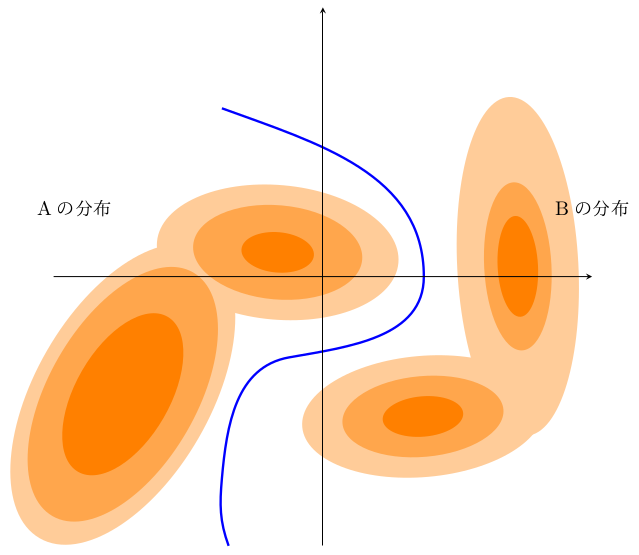
\includegraphics[width=6cm]{senkei.png}};
    \draw[very thick,->] (-6,0)--(6,0) node[right]{$y$};
    \draw[very thick,->] (-0.5,-0.3)--(-0.5,3.5);
    %%
    \fill[fill=blue] (-4,4.5) circle[radius=0.1];
    \fill[fill=blue] (-2,5) circle[radius=0.1];
    \fill[fill=red] (-6.8,4.5) circle[radius=0.1];
    \fill[fill=red] (-5,5.2) circle[radius=0.1];
    %%
    \draw[xscale=1.5,domain=0:6,thick,draw=green] plot(\x-3,{3/(1+exp(-3*\x+8))});
    \draw[draw=gray!40](-6,3)--(6,3);
    \fill[fill=red] (-5,0) circle[radius=0.1];
    \fill[fill=red] (-2.5,0) circle[radius=0.1];
    \fill[fill=blue] (1.5,3) circle[radius=0.1];
    \fill[fill=blue] (4,3) circle[radius=0.1];
    \draw[fill=white,draw=blue] (1.5,0) circle[radius=0.1];
    \draw[fill=white,draw=blue] (4,0) circle[radius=0.1];
    \draw[<->] (1.5,0.1)--(1.5,2.9);
    \draw[<->] (4,0.1)--(4,2.9);

    \draw[->,draw=gray!80] (-6.8,4.4) to [out=270,in=180] (-5.5,3) to[out=0,in=90] (-5,0.1);
    \draw[->,draw=gray!80] (-5,5.1) to [out=270,in=180] (-4,3.2) to[out=0,in=90] (-2.5,0.1);
    \draw[->,draw=gray!80] (-3.9,4.5) to[out=0,in=120] (1.43,0.14);
    \draw[->,draw=gray!80] (-1.9,5) to[out=0,in=110] (3.94,0.14);
  \end{tikzpicture}
\end{center}
\begin{eqnarray*}
  z=f(y;\Psi) = f(g(x;\Theta);\Psi)
\end{eqnarray*}
線形識別の場合は
\begin{center}
  \begin{tikzpicture}[>=stealth,scale=1.2]
        \fill[fill=orange!40,rotate=60] (-3,1.7) circle[xscale=1.9,radius=1.3];
        \fill[fill=orange!40,rotate=-5] (-0.7,0.3) circle[xscale=1.8,radius=1];
        \fill[fill=orange!70,rotate=60] (-3,1.7) circle[xscale=1.9,radius=1.1];
        \fill[fill=orange!70,rotate=-5] (-0.7,0.3) circle[xscale=1.8,radius=0.7];
        \fill[fill=orange,rotate=60] (-3,1.7) circle[xscale=1.9,radius=0.7];
        \fill[fill=orange,rotate=-5] (-0.7,0.3) circle[xscale=1.8,radius=0.3];

        \fill[fill=orange!40,rotate=93] (0,-2.9) circle[xscale=2.8,radius=0.9];
        \fill[fill=orange!40,rotate=5] (1.3,-2.2) circle[xscale=2,radius=0.9];
        \fill[fill=orange!70,rotate=93] (0,-2.9) circle[xscale=2.5,radius=0.5];
        \fill[fill=orange!70,rotate=5] (1.3,-2.2) circle[xscale=2,radius=0.6];
        \fill[fill=orange,rotate=93] (0,-2.9) circle[xscale=2.5,radius=0.3];
        \fill[fill=orange,rotate=5] (1.3,-2.2) circle[xscale=2,radius=0.3];
        \draw[->] (-4,0)--(4,0);
        \draw[->] (0,-4)--(0,4);
        \fill[fill=red] (0.2,0.3) circle[radius=0.1];
        \fill[fill=red] (-1,0.35) circle[radius=0.1];
        \fill[fill=red] (-1.5,-0.35) circle[radius=0.1];
        \fill[fill=red] (-1.9,-0.5) circle[radius=0.1];
        \fill[fill=red] (-3,-1) circle[radius=0.1];
        \fill[fill=red] (-3.5,-2) circle[radius=0.1];
        \fill[fill=red] (-3.2,-1.7) circle[radius=0.1];
        \fill[fill=red] (-2.7,-3) circle[radius=0.1];
        \fill[fill=red] (-3.6,-3.5) circle[radius=0.1];
        %%
        \fill[fill=blue] (-0.1,-2.2) circle[radius=0.1];
        \fill[fill=blue] (0.1,-2.4) circle[radius=0.1];
        \fill[fill=blue] (0.7,-1.9) circle[radius=0.1];
        \fill[fill=blue] (1.3,-1.5) circle[radius=0.1];
        \fill[fill=blue] (1.3,-2.5) circle[radius=0.1];
        \fill[fill=blue] (2.3,-0.5) circle[radius=0.1];
        \fill[fill=blue] (2.5,-1) circle[radius=0.1];
        \fill[fill=blue] (3.2,-0.3) circle[radius=0.1];
        \fill[fill=blue] (3,0.8) circle[radius=0.1];
        \fill[fill=blue] (3,2.2) circle[radius=0.1];
        \fill[fill=blue] (3.1,-2) circle[radius=0.1];
        \node at(-3.7,1) {Aの分布};
        \node at(4,1) {Bの分布};
        \draw[very thick,draw=blue] (-1.3,3)--(1.5,-4.5);
        \draw[very thick,draw=blue] (-2,-5)--(6,-2);
        \node at(6.2,-2) {$y$};
    \end{tikzpicture}
  \end{center}
  入力データ($x_{i}$)に対して線形識別における座標変換すると
  \begin{eqnarray*}
  y_{i}=\mbox{\boldmath $w$}^{T}\mbox{\boldmath $x$}_{i}  
  \end{eqnarray*}
  これに対してロジスティック回帰を適用させると
  \begin{align*}
    z_{i}=\frac{1}{1+{\rm exp}(-y_{i})}= \frac{1}{1+{\rm exp}(-\mbox{\boldmath $w$}^{T}\mbox{\boldmath $x$}_{i})} \tag{4.1}
  \end{align*}
  以下の2層のニューラルネット(パーセプトロン)について考える.
  \begin{center}
    \begin{tikzpicture}[>=stealth]
      \draw(0,0) circle[radius=0.3];
      \draw(-2,0) circle[radius=0.3];
      \draw(2,0) circle[radius=0.3];
      \draw(-4,0) circle[radius=0.3];
      \draw(4,0) circle[radius=0.3];
      \draw(0,4) circle[radius=0.3];
      \draw[->](0,0.3)--(0,3.7);
      \draw[->] (1.85,0.25)--(0.15,3.76);
      \draw[->] (-1.85,0.25)--(-0.15,3.76);
      \draw[->] (3.8,0.2)--(0.25,3.82);
      \draw[->] (-3.8,0.2)--(-0.25,3.82);
      \draw[->] (0,4.3)--(0,5.2);
      \node at(-4,-0.7) {$x_{1}$};
      \node at(-2,-0.7) {$x_{2}$};
      \node at(0,-0.7) {$x_{3}$};
      \node at(1,-0.7) {$\cdots$};
      \node at(2,-0.7) {$x_{i}$};
      \node at(3,-0.7) {$\cdots$};
      \node at(4,-0.7) {$x_{N}$};
      \node at(-3,2) {$w_{1}$};
      \node at(-1,2) {$w_{2}$};
      \node at(0,2) {$w_{3}$};
      \node at(1,2) {$w_{i}$};
      \node at(2.5,2) {$w_{N}$};
      \node at(0.5,2) {$\cdots$};
      \node at(1.65,2) {$\cdots$};
    \end{tikzpicture}
  \end{center}
  $\mbox{\boldmath $x$}^{(k)}=\begin{pmatrix} x_{1}^{(k)}&x_{2}^{(k)}&\cdots&x_{i}^{(k)}&\cdots&x_{N}^{(k)}\end{pmatrix}^{T}$\ :\ 第$k$入力ベクトル\\
  $y^{(k)}$\ :\ 第$k$に対する出力
  \begin{eqnarray*}
    &&y^{(k)}=f\left(\sum_{i=1}^{N}w_{i}x_{i}^{(k)}\right)\\
    &&f(z)=\frac{1}{1+{\rm exp}(-z)}
  \end{eqnarray*}
  カテゴリ$A$であれば1, そうでなければ0とする.\ また\\
  $\mbox{\boldmath $w$}=\begin{pmatrix}w_{1}&w_{2}&\cdots&w_{i}&\cdots&w_{N}\end{pmatrix}$\ :\ 重みベクトル(パーセプトロンのパラメータ)\\
  $t^{(k)}$\ :\ 第$k$入力に対する正解カテゴリ(カテゴリ$A$であれば1そうでなければ0)\\
  $M$\ :\ データの個数\\
  目的関数$H(\mbox{\boldmath $w$})$としたとき目的関数の中身は以下のようになる。
  \begin{eqnarray*}
    H(\mbox{\boldmath $w$})&=&\sum_{j = 1}^{M}\frac{1}{2}\left(y^{(j)}-t^{(j)}\right)^{2}\\
    &=&\sum_{j=1}^{M}\frac{1}{2}\left(f\left(\sum_{i=1}^{N}w_{i}x_{i}{}^{(j)}\right)-t^{(j)}\right)^{2}, f(z)=\frac{1}{1+e^{-z}}\\
  \end{eqnarray*}
  この時最急降下法により、$\mbox{\boldmath $w$}$を求めると次のようになる。\\
  まず更新式は次のようにあらわされる。
  \begin{eqnarray*}
    \mbox{\boldmath $w$}_{n+1}=\mbox{\boldmath $w$}_{n}-\alpha_{n}\frac{\mathrm{\partial} H\left(\mbox{\boldmath $w$}_{n}\right)}{\mathrm{\partial} \mbox{\boldmath $w$}}\\
    \alpha_{n+1}=\beta\alpha_{n}, \alpha_{0}=0.5,\beta=0.98
  \end{eqnarray*}
  ここで、以下の性質が成り立つ
  \begin{eqnarray*}
    H(\mbox{\boldmath $w$})=\sum_{j=1}^{M}\frac{1}{2}\left(y^{(j)}-t^{(j)}\right)^{2},\\
    y^{(j)}=f\left(\sum_{i=1}^{N}w_{i}x_{i}{}^{(j)}\right)\text{の時}\\
    \frac{\mathrm{\partial}}{\mathrm{\partial} w_{i}}H(\mbox{\boldmath $w$})=\sum_{j=1}^{M}\left(y^{(j)}-t^{(j)}\right)y^{(j)}\left(1-y^{(j)}\right)x_{i}{}^{(j)}
  \end{eqnarray*}
  よって、次のことが成り立つ
  \begin{eqnarray*}
    \nabla H(\mbox{\boldmath $w$})
    &=&\frac{\mathrm{\partial}H(\mbox{\boldmath $w$})}{\mathrm{\partial}\mbox{\boldmath $w$}}\\
    &=&[H(\mbox{\boldmath $w$})]% &=&[]
  \end{eqnarray*}
\section{ニューラルネットワークと確率降下法}
入力-出力の対($\mbox{\boldmath $x$},\ \mbox{\boldmath $y$}$)が大量に与えられば, 関数$y=f(x)$を精度よくもとめることができる.
\section{情報圧縮と等式制約の最適化問題}
情報圧縮の典型的問題は主成分分析である. 情報圧縮する必要性として, 特徴空間の
次元が高くなると, 信頼できる境界を得るために必要な学習データの量が幾何級数的に増大するためである.\\
つまり次元を増やすたびに, 周囲にクラスを定めていない未知の空間が幾何級数的に増加するということである.
\begin{center}
    \begin{tikzpicture}[>=stealth]
    \draw[->](0,0)--(4,0);
    \filldraw[fill=blue] (1,0) circle[radius=0.1];
    \filldraw[fill=green] (3,0) circle[radius=0.1];
    \end{tikzpicture}
\end{center}
\begin{center}
    \begin{tikzpicture}[>=stealth]
    \draw[->](0,0)--(4,0);
    \draw[->](2,0.5)--(0,-1.5);
    \filldraw[fill=blue] (1,0) circle[radius=0.1];
    \filldraw[fill=green] (3,0) circle[radius=0.1];
    \end{tikzpicture}
\end{center}
\begin{center}
    \begin{tikzpicture}[>=stealth]
    \draw[->](0,0)--(4,0);
    \draw[->](2,0.5)--(0,-1.5);
    \draw[->](1.5,-0.8)--(1.5,2);
    \filldraw[fill=blue] (1,0) circle[radius=0.1];
    \filldraw[fill=green] (3,0) circle[radius=0.1];
    \end{tikzpicture}
\end{center}
\begin{itemize}
    \item 情報圧縮\\
    高次元空間上のデータを, 低次元の空間に, ある基準のもとで写像する
    \item 主成分分析\\
    低次元への写像に伴う情報のロスを最小に抑える線形写像
\end{itemize}
\subsection{主成分分析}
以下のように$R^{2}$の空間に分布するデータが与えられたとする.
\begin{center}
    \begin{tikzpicture}
        \draw[dashed](0,0) grid (10,6);
        \fill[fill=blue](2.2,3.8) circle [radius=0.1];
        \fill[fill=blue](2.8,4.5) circle [radius=0.1];
        \fill[fill=blue](3.2,3.7) circle [radius=0.1];
        \fill[fill=blue](3.3,2.7) circle [radius=0.1];
        \fill[fill=blue](3.8,4.7) circle [radius=0.1];
        \fill[fill=blue](4,4) circle [radius=0.1];
        \fill[fill=blue](4.5,4.4) circle [radius=0.1];
        \fill[fill=blue](4.5,3.8) circle [radius=0.1];
        \fill[fill=blue](4.5,3) circle [radius=0.1];
        \fill[fill=blue](4.5,1.7) circle [radius=0.1];
        \fill[fill=blue](4.8,2.5) circle [radius=0.1];
        \fill[fill=blue](5.3,1.4) circle [radius=0.1];
        \fill[fill=blue](5.5,3.7) circle [radius=0.1];
        \fill[fill=blue](5.7,2.8) circle [radius=0.1];
        \fill[fill=blue](6,2) circle [radius=0.1];
        \fill[fill=blue](6.3,0.8) circle [radius=0.1];
        \fill[fill=blue](6.7,2.7) circle [radius=0.1];
        \fill[fill=blue](6.9,2) circle [radius=0.1];
        \fill[fill=blue](7,1.3) circle [radius=0.1];
        \fill[fill=blue](7.7,2.1) circle [radius=0.1];
    \end{tikzpicture}
\end{center}
この空間上に分布するデータを, 直線状の部分空間に写像することを考える. すると以下のような写像が考えられる.
\begin{center}
    \begin{tikzpicture}
        \draw[draw=green,dashed] (2.8,4.5)--(2.55,3.64);
        \draw[draw=green,dashed] (3.8,4.7)--(3.4,3.38);
        \draw[draw=green,dashed] (4.5,1.7)--(4.85,2.93);
        \draw[dashed](0,0) grid (10,6);
        \fill[fill=blue](2.2,3.8) circle [radius=0.1];
        \fill[fill=blue](2.8,4.5) circle [radius=0.1];
        \fill[fill=blue](3.2,3.7) circle [radius=0.1];
        \fill[fill=blue](3.3,2.7) circle [radius=0.1];
        \fill[fill=blue](3.8,4.7) circle [radius=0.1];
        \fill[fill=blue](4,4) circle [radius=0.1];
        \fill[fill=blue](4.5,4.4) circle [radius=0.1];
        \fill[fill=blue](4.5,3.8) circle [radius=0.1];
        \fill[fill=blue](4.5,3) circle [radius=0.1];
        \fill[fill=blue](4.5,1.7) circle [radius=0.1];
        \fill[fill=blue](4.8,2.5) circle [radius=0.1];
        \fill[fill=blue](5.3,1.4) circle [radius=0.1];
        \fill[fill=blue](5.5,3.7) circle [radius=0.1];
        \fill[fill=blue](5.7,2.8) circle [radius=0.1];
        \fill[fill=blue](6,2) circle [radius=0.1];
        \fill[fill=blue](6.3,0.8) circle [radius=0.1];
        \fill[fill=blue](6.7,2.7) circle [radius=0.1];
        \fill[fill=blue](6.9,2) circle [radius=0.1];
        \fill[fill=blue](7,1.3) circle [radius=0.1];
        \fill[fill=blue](7.7,2.1) circle [radius=0.1];
        \draw[draw=green] (1.4,4)--(8.8,1.7);
        \fill[fill=green] (2.2,3.75) circle[radius=0.1];
        \fill[fill=green] (2.55,3.64) circle[radius=0.1];
        \fill[fill=green] (3.1,3.47) circle[radius=0.1];
        \fill[fill=green] (3.4,3.38) circle[radius=0.1];
        \fill[fill=green] (3.6,3.32) circle[radius=0.1];
        \fill[fill=green] (3.8,3.25) circle[radius=0.1];
        \fill[fill=green] (4.1,3.16) circle[radius=0.1];
        \fill[fill=green] (4.3,3.10) circle[radius=0.1];
        \fill[fill=green] (4.5,3.04) circle[radius=0.1];
        \fill[fill=green] (4.8,2.94) circle[radius=0.1];
        \fill[fill=green] (5.2,2.82) circle[radius=0.1];
        \fill[fill=green] (5.6,2.69) circle[radius=0.1];
        \fill[fill=green] (5.7,2.66) circle[radius=0.1];
        \fill[fill=green] (6.2,2.51) circle[radius=0.1];
        \fill[fill=green] (6.5,2.41) circle[radius=0.1];
        \fill[fill=green] (6.7,2.35) circle[radius=0.1];
        \fill[fill=green] (7,2.26) circle[radius=0.1];
        \fill[fill=green] (7.25,2.18) circle[radius=0.1];
        \fill[fill=green] (7.7,2.04) circle[radius=0.1];
        \filldraw[fill=magenta] (5,2.88) circle[radius=0.1];
    \end{tikzpicture}
\end{center}
\begin{center}
    \begin{tikzpicture}[>=stealth]
        \draw[draw=green,dashed] (2.8,4.5)--(2.55,3.64);
        \draw[draw=green,very thick] (3.8,4.7)--(3.4,3.38);
        \draw[draw=green,dashed] (4.5,1.7)--(4.85,2.93);
        \draw[dashed](0,0) grid (10,6);
        \fill[fill=blue](2.2,3.8) circle [radius=0.1];
        \fill[fill=blue](2.8,4.5) circle [radius=0.1];
        \fill[fill=blue](3.2,3.7) circle [radius=0.1];
        \fill[fill=blue](3.3,2.7) circle [radius=0.1];
        \filldraw[fill=blue](3.8,4.7) circle [radius=0.15];
        \fill[fill=blue](4,4) circle [radius=0.1];
        \fill[fill=blue](4.5,4.4) circle [radius=0.1];
        \fill[fill=blue](4.5,3.8) circle [radius=0.1];
        \fill[fill=blue](4.5,3) circle [radius=0.1];
        \fill[fill=blue](4.5,1.7) circle [radius=0.1];
        \fill[fill=blue](4.8,2.5) circle [radius=0.1];
        \fill[fill=blue](5.3,1.4) circle [radius=0.1];
        \fill[fill=blue](5.5,3.7) circle [radius=0.1];
        \fill[fill=blue](5.7,2.8) circle [radius=0.1];
        \fill[fill=blue](6,2) circle [radius=0.1];
        \fill[fill=blue](6.3,0.8) circle [radius=0.1];
        \fill[fill=blue](6.7,2.7) circle [radius=0.1];
        \fill[fill=blue](6.9,2) circle [radius=0.1];
        \fill[fill=blue](7,1.3) circle [radius=0.1];
        \fill[fill=blue](7.7,2.1) circle [radius=0.1];
        \draw[draw=green] (1.4,4)--(8.8,1.7);
        \fill[fill=green] (2.2,3.75) circle[radius=0.1];
        \fill[fill=green] (2.55,3.64) circle[radius=0.1];
        \fill[fill=green] (3.1,3.47) circle[radius=0.1];
        \filldraw[fill=green] (3.4,3.38) circle[radius=0.15];
        \fill[fill=green] (3.6,3.32) circle[radius=0.1];
        \fill[fill=green] (3.8,3.25) circle[radius=0.1];
        \fill[fill=green] (4.1,3.16) circle[radius=0.1];
        \fill[fill=green] (4.3,3.10) circle[radius=0.1];
        \fill[fill=green] (4.5,3.04) circle[radius=0.1];
        \fill[fill=green] (4.8,2.94) circle[radius=0.1];
        \fill[fill=green] (5.2,2.82) circle[radius=0.1];
        \fill[fill=green] (5.6,2.69) circle[radius=0.1];
        \fill[fill=green] (5.7,2.66) circle[radius=0.1];
        \fill[fill=green] (6.2,2.51) circle[radius=0.1];
        \fill[fill=green] (6.5,2.41) circle[radius=0.1];
        \fill[fill=green] (6.7,2.35) circle[radius=0.1];
        \fill[fill=green] (7,2.26) circle[radius=0.1];
        \fill[fill=green] (7.25,2.18) circle[radius=0.1];
        \fill[fill=green] (7.7,2.04) circle[radius=0.1];
        \draw[very thick,->] (5,2.88)--(3.8,4.7);
        \draw[very thick,->] (5,2.88)--(3.4,3.38);
        \filldraw[fill=magenta] (5,2.88) circle[radius=0.15];
        \node at(2.8,2.8) {$A'$};
        \node at(3.75,5.2) {$A$};
    \end{tikzpicture}
\end{center}
このとき$A-A'$がロスとなる. $A'$において射影成分の分散が最大化されるように直線を引く時, これはロスが最小化されることとなる. これはOAの距離が一定であるので, $A-A'$の値が最小となるときは$O-A'$の値が最大となるためである.部分空間が変われば, 分散も変わるので, 最も射影成分の分散の大きくなる部分空間を求めることがよい. \\
次に第1主成分の求め方について扱う.\\
いま$P$次元のベクトルが,$N$個あるとする.
\begin{eqnarray*}
    \mbox{\boldmath $x$}_{n}=\begin{pmatrix}x_{np}\end{pmatrix},\ (p=1,2,3,\cdots,P)\ (n=1,2,3,\cdots,N)
\end{eqnarray*}
簡単のため, 各変数についてその平均値を0とする. 0ではない場合は平均値を引いて新たに変数を定義しなおせば一般性は失われない.\\
ここで, 測定データ全体は次の行列$X$で与えられる.
\begin{eqnarray*}
    X=\begin{pmatrix} \mbox{\boldmath $x$}_{1}&\mbox{\boldmath $x$}_{2}&\cdots&\mbox{\boldmath $x$}_{n}\end{pmatrix}^{T}=\begin{pmatrix} x_{11}&x_{12}&\cdots&x_{1P}\\ x_{21}&x_{22}&\cdots&x_{2P}\\\vdots&\vdots&\ddots&\vdots \\ x_{N1}&x_{N2}&\cdots&x_{NP} \end{pmatrix}
\end{eqnarray*}
求める主成分を
\begin{eqnarray*}
    \mbox{\boldmath $w$} = \begin{pmatrix}w_{1}&w_{2}&\cdots&w_{P}\end{pmatrix}^{T}\ \|\mbox{\boldmath $w$}\|=\mbox{\boldmath $w$}^{T}\mbox{\boldmath $w$}=1
\end{eqnarray*}
とし, 今$n$番目のデータを
\begin{eqnarray*}
    \mbox{\boldmath $x$}_{n}=\begin{pmatrix} x_{n1}&x_{n2}&\cdots&x_{nP}\end{pmatrix}^{T}
\end{eqnarray*}
の主成分への射影$z_{n}$を考えると,
\begin{eqnarray*}
    z_{n}=\mbox{\boldmath $x$}_{n}^{T}\mbox{\boldmath $w$}=\sum_{p=1}^{P}x_{np}w_{p}
\end{eqnarray*}
$\mbox{\boldmath $z$}=\begin{pmatrix}z_{1}&z_{2}&\cdots &z_{N}\end{pmatrix}^{T}$とすれば,
\begin{eqnarray*}
    \mbox{\boldmath $z$}=X\mbox{\boldmath $w$}
\end{eqnarray*}
このとき$z_{n}$の分散$\sigma^{2}$は
\begin{eqnarray*}
    \sigma^{2}&=&\frac{1}{N}\bm{z}^{T}\bm{z}=\frac{1}{N}(X\bm{w})^{T}(X\bm{w})\\
            &=&\frac{1}{N}\bm{w}^{T}X^{T}X\bm{w}=\bm{w}^{T}C\bm{w}
\end{eqnarray*}
ただし,
\begin{eqnarray*}
    C=\{c_{ij}\},\ c_{ij}=\frac{1}{N}\sum_{k=1}^{N}x_{ki}x_{kj}
\end{eqnarray*}
$C$は, 共分散行列とよばれ, 平均値が0でない一般的な場合は
\begin{eqnarray*}
    c_{ij}=\frac{1}{N}\sum_{k=1}^{N}(x_{ki}-{x_{i}})(x_{kj}-\bar{x_{j}})
\end{eqnarray*}
となる.\ ここで, 第1主成分は$\bm{w}$で$\sigma^{2}$の最大化すること. つまり
\begin{eqnarray*}
    \underset{\bm{w}}{\rm max}\bm{w}^{T}C\bm{w}
\end{eqnarray*}
を満たすことである. この中で条件として$\bm{w}^{T}\bm{w}=1$を満たさなければならない. 定式化すると
\begin{eqnarray*}
    \underset{\bm{w}}{\rm max}\bm{w}^{T}C\bm{w}\\
    s.t.\ \ \bm{w}^{T}\bm{w}=1
\end{eqnarray*}
\subsection{Lagrangeの未定乗数法}
以下の問題を求める方法である.
\begin{eqnarray*}
    \underset{x}{\rm max}f(\bm{x})\\
    s.t.\ g(\bm{x})=0
\end{eqnarray*}
一般的な解法として
\begin{align*}
   L(\bm{x})=f(\bm{x})+\lambda g(\bm{x}) \tag{6.1}
\end{align*}
とおき,
\begin{eqnarray*}
    \left\{
    \begin{array}{l}
      \displaystyle \frac{\partial}{\partial \bm{x}}L(\bm{x}) = 0\\
      g(\bm{x})=0
    \end{array}
    \right.
\end{eqnarray*}
の連立方程式を解くことである.\\
\begin{screen}
周囲の長さがXの長方形の中で, 面積の一番大きいものの辺の長さを求める.\\
各辺を$a,\,b$とおくと問題は
    \begin{eqnarray*}
        {\rm max}&& ab\\
        && s.t.\ 2(a+b)=X
    \end{eqnarray*}
    という問題となる.\\
    つまり, \\
    \begin{eqnarray*}
        f(a,b) &=& ab\\
        g(a,b) &=& 2(a+b)-X
    \end{eqnarray*}
    となるので,
    \begin{eqnarray*}
        L(a,b,\lambda) &=& f(a,b)- \lambda g(a,b)\\
                        &=& ab - \lambda (2a+2b-X)
    \end{eqnarray*}
    について連立方程式を立てて解けばよい.
    \begin{eqnarray*}
        && \frac{\partial}{\partial a} L (a,b,\lambda) = b-2\lambda = 0\\
        && \frac{\partial}{\partial b} L (a,b,\lambda) = a-2\lambda = 0\\
        && \frac{\partial}{\partial \lambda} L(a,b,\lambda) = -2a-2b+X = 0
    \end{eqnarray*}
    となるので, 整理すると
    \begin{eqnarray*}
        && a = b = \lambda\\
        && -4\lambda-4\lambda+X = 0\\
        && \lambda = \frac{X}{8}\\
        && a=b=2\lambda = \frac{X}{4}
    \end{eqnarray*}
となる.
\end{screen}
Lagrangeの未定乗数法を用いて$\bm{w}$による$\sigma^{2}$の最大化問題は$\|\bm{w}\|=\bm{w}^{T}\bm{w}=1$の条件の下で解くことを考える.\\
Lagrangeの未定乗数法より以下の方程式を立てる.
\begin{eqnarray*}
    L(\bm{w},\lambda)=\bm{w}^{T}C\bm{w}-\lambda(\bm{w}^{T}\bm{w}-1)
\end{eqnarray*}
とおいて, $\displaystyle \frac{\partial L}{\partial \bm{w}}=0$を解くことを考える. すると
\begin{eqnarray*}
    \frac{\partial L}{\partial \bm{w}}&=&C\bm{w}+(\bm{w}^{T}C)^{T}-\lambda(\bm{w}+\bm{w})\\
                                      &=&C\bm{w}+C^{T}\bm{w}-2\lambda \bm{w}\\
                                      &=&C\bm{w}+C\bm{w}-2\lambda \bm{w}\\
                                      &=&2(C-\lambda I)\bm{w} = 0
\end{eqnarray*}
となる. 共分散行列に関して
\begin{eqnarray*}
    c_{ij}=\frac{1}{N}\sum_{k=1}^{N}x_{ki}x_{kj} = \frac{1}{N}\sum_{k=1}^{N}x_{kj}x_{ki} = c_{ji}
\end{eqnarray*}
であるから, 対称行列であることがいえる. よって,
\begin{eqnarray*}
    (C-\lambda I)\bm{w} = 0 \ \Longleftrightarrow\ C\bm{w} = \lambda \bm{w}
\end{eqnarray*}
となり, 問題は固有値問題に帰着される.\\
また
\begin{eqnarray*}
    (C-\lambda I)\bm{w} = 0 \ \Longleftrightarrow\ {\rm det}|C-\lambda I|=0
\end{eqnarray*}
となるので, $\lambda$が満たすべき条件は, 共分散行列$C$の固有方程式となる.\\
したがって, 射影の分散の最大値を与える主成分$\bm{w}$は分散共分散行列の固有ベクトルのひとつであり, $\lambda$はその固有ベクトルに対応した固有値であることがわかる.\\
データ数が$P$個あることから$(C-\lambda I)\bm{w}=0$を満たす固有ベクトル$\bm{w}$, 固有値$\lambda$はそれぞれ$P$個ある.\\
このうち, どれが射影の分散の最大値を与えるかを考える.
\begin{eqnarray*}
    C\bm{w} = \lambda \bm{w}
\end{eqnarray*}
という関係の下,
\begin{eqnarray*}
    \sigma^{2}=\bm{w}^{T}C\bm{w}
\end{eqnarray*}
であるから
\begin{eqnarray*}
    \sigma^{2}=\bm{w}^{T}C\bm{w}=\lambda \bm{w}^{T}\bm{w}
\end{eqnarray*}
となり,\,$\bm{w}^{T}\bm{w}=1$であることを考慮すれば
\begin{eqnarray*}
    \sigma^{2}=\lambda
\end{eqnarray*}
となる. つまり\textcolor{red}{射影の分散の値は固有値に等しい}.\\
よって, 求める主成分は最大固有値に対応した固有ベクトルとして与えられることが分かる.\\[1cm]
第2以降の主成分の求め方について,\\
帰納的に第$m$主成分を求める. 分散共分散行列$C$の固有値のうち大きいものから順に$m-1$個に対応する固有ベクトルとして, $m-1$の主成分$\bm{w}_{1},\bm{w}_{2},\cdots ,\bm{w}_{k},\cdots,\bm{w}_{m-1}$が求まっているとする. これらのベクトルは
\begin{eqnarray*}
    &&(C-\lambda I)\bm{w}_{k}=0\\
    &&\bm{w}_{k}^{T}\bm{w}_{k}=1
\end{eqnarray*}
を満たし, 互いに直交しているものとする\footnote{$\bm{w}$は固有ベクトルなので自明}.
\begin{eqnarray*}
    \bm{w}_{k}^{T}\bm{w}_{k'(\neq k)}=0
\end{eqnarray*}
つまり
\begin{eqnarray*}
    f(\bm{w}_{m}) = \bm{w}_{m}^{T}C\bm{w}_{m}\\
    s.t.\ \bm{w}_{m}^{T}\bm{w}_{m}=1,\ \bm{w}_{k}^{T}\bm{w}_{k'(k'\neq k)}=0
\end{eqnarray*}
という関係式が得られる.\\
Lagrangeの未定乗数法より
\begin{align*}
    J_{m}=\bm{w}_{m}^{T}C\bm{w}_{m}-\lambda_{m}(\bm{w}_{m}^{T}\bm{w}_{m}-1)-\sum_{k=1}^{m-1}\mu_{k}\bm{w}_{m}^{T}\bm{w}_{k}
\end{align*}
とおいて, $\displaystyle \frac{\partial J_{m}}{\partial \bm{w}_{m}}=0$とおくと,
\begin{eqnarray*}
    &&2C_{\bm{w}_{m}}-2\lambda_{m}\bm{w}-\sum_{k=1}^{m-1}\mu_{k}\bm{w}_{k}=0\\
   \Longleftrightarrow\ && C_{\bm{w}}-\lambda_{m}\bm{w}_{m}-\sum_{k=1}^{m-1}\mu_{k}\bm{w}_{k}=0
\end{eqnarray*}
ここで$\mu_{k}$について$\mu_{k}=\frac{1}{2}\mu_{k}$として再定義.\\
左から$\bm{w}_{j}^{T}\,(j=1,2,3,\cdots,m-1)$をかけると,($\bm{w}_{k}^{T}\bm{w}_{k'(k' \neq k)}=0$を考慮して)
\begin{eqnarray*}
&&\bm{w}_{j}^{T}C\bm{w}_{m}-\lambda_{m}\bm{w}_{j}^{T}\bm{w}_{m}-\sum_{k=1}^{m-1}\mu_{k}\bm{w}_{j}\bm{w}_{k}=0\\
    \Longleftrightarrow \ && \bm{w}_{j}^{T}C\bm{w}_{m}-\mu_{j}=0
\end{eqnarray*}
となる. また
\begin{eqnarray*}
    \bm{w}_{j}^{T}C\bm{w}_{m}&=&\bm{w}_{m}^{T}C\bm{w}_{j}\\
                             &=&\lambda_{j}\bm{w}_{m}^{T}\bm{w}_{j}=0\ (j=1,2,\cdots,m-1)
\end{eqnarray*}
であることから
\begin{eqnarray*}
    \mu_{j}=0\ (j=1,2,\cdots,m-1)
\end{eqnarray*}
となる. これから最適化のための評価関数として以下の関係式が導かれる.
\begin{align*}
    J_{m}=\bm{w}_{m}^{T}C\bm{w}_{m}\lambda_{m}(\bm{w}_{m}^{T}\bm{w}_{m}-1) \tag{6.2}
\end{align*}
よって, 第1主成分を求めるための評価関数と同じであるから, 求める第$m$主成分$\bm{w}_{m}$は\textcolor{red}{分散共分散行列の$C$の$m$番目に大きい固有値に対応した固有ベクトルとして与えられる}.\\[1cm]
\begin{itemize}
  \item 寄与率\ :\ 部分空間で表現出来る分布の広がり程度\\
    -元の空間における分散\ :\ $\sigma_{O}^{2}$\\
    -第$m$時の部分空間における分散\ :\ $\sigma_{Sm}^{2}$\\
    とすると
    \begin{align*}
      寄与率=\frac{\sigma_{Sm}^{2}}{\sigma_{O}^{2}} \tag{6.3}
    \end{align*}
    となる.
  \item 累積寄与率
    \begin{align*}
      累積寄与率=\frac{\sum_{m=1}^{M}\sigma_{Sm}^{2}}{\sigma_{O}^{2}} \tag{6.4}
    \end{align*}
\end{itemize}
\subsection{線形判別分析(LDA:Linear Discriminant Analysis}
級内分散$C_{W}$と級間分散$C_{B}$の比を最大にする座標空間を求める.
\begin{center}
    \begin{tikzpicture}[>=stealth,scale=2]
        \fill[fill=green!40] (0.1,0.1) circle[radius=0.7];
        \fill[fill=magenta!40] (3.3,0.9) circle[radius=0.7];
        \draw(0,0)--(3,1);
        \draw(0,0)--(3.8,0.63);
        \draw[thick,red,->] (0,0)--(-0.8,-0.266);
        \draw[thick,red,->] (0,0)--(-1.1,-0.183);
        \draw[thick,red,->] (3,1)--(3.8,1.266);
        \draw[thick,red,->] (3.8,0.63)--(4.6,0.766);
        \draw (-0.15,0.075)--(0.6,-0.3);
        \draw (-0.08,0.16)--(0.25,-0.5);
        \draw[->,draw=blue,thick] (0,0)--(0.1,-0.2);
        \draw[->,draw=blue,thick] (0.2,-0.4)--(0.1,-0.2);
        \draw[->,draw=blue,thick] (0,0)--(0.22,-0.11);
        \draw[->,draw=blue,thick](0.5,-0.25)--(0.28,-0.14);
        \draw (2.8,1.0925)--(4,0.5375);
        \draw[->,draw=blue,thick] (3,1)--(3.4,0.815);
        \draw[->,draw=blue,thick] (3.8,0.63)--(3.4,0.815);
        \filldraw[fill=white] (0,0) circle[radius=0.05];
        \filldraw[fill=white] (3,1) circle[radius=0.05];
        \filldraw[fill=white] (3.8,0.63) circle[radius=0.05];
        \filldraw[fill=white] (0.2,-0.4) circle[radius=0.05];
        \filldraw[fill=white] (0.5,-0.25) circle[radius=0.05];
    \end{tikzpicture}
\end{center}
カテゴリの同じデータは近くに, 違うデータは遠くに配置する.\\
2クラスの場合のLDAについて考えてみる. 2クラスについてそれぞれクラス$A,\,B$として以下の関数について考えてみる.\\
$y=\bm{w}^{T}\bm{x}$\\
$\mu'=E[y],\ \sigma'=E[(y-\mu)^{2}]$\\
として
\begin{eqnarray*}
    J(\bm{w})=\frac{(\mu_{A}'-\mu_{B}')^{2}}{\sigma_{A}'^{2}+\sigma_{B}'^{2}}
\end{eqnarray*}
射影ベクトル$\bm{w}$を変えると$J$の値が変わると, $J$が大きい時, 違うデータの集まりが遠くに配置されていることになるので, 識別が容易になる.\ したがって, $J$を最大化するベクトル$\bm{w}$を求めることでクラスを分割することができる.\\
$\bm{x}$\ :\ 特徴ベクトル\\
$n_{i}$\ :\ クラス$i$のデータ数$\displaystyle \left(総データ数 n=\sum_{i}n_{i}\right)$\\
$\bm{\mu}_{i}$\ :\ クラス$i$の平均ベクトル\\
$X_{i}$\ :\ クラス$i$に対する元空間における特徴ベクトルの集合\\
とおくと,
$C_{i}$\ :\ クラス$i$の共分散行列\\
$S_{i}$\ :\ クラス$i$の変動行列\\
は次式で定義される.
\begin{eqnarray*}
    C_{i}&=&\frac{1}{n_{i}}\sum_{\bm{x}\in X_{i}}(\bm{x}-\bm{\mu}_{i})(\bm{x}-\bm{\mu}_{i})^{T}\\
    S_{i}&=&\sum_{\bm{x}\in X_{i}}(\bm{x}-\bm{\mu}_{i})(\bm{x}-\bm{\mu}_{i})^{T}=n_{i}C_{i}
\end{eqnarray*}
また, 射影先について考える.ベクトル$\bm{w}$に$\bm{x}$を射影して作った1次元の空間において\\
$y$\ :\ 射影して作られた$\bm{x}$の像\ $y=\bm{w}^{T}\bm{x}$\\
$\tilde{\mu_{i}}$\  :\ 射影先の空間におけるクラス$i$のデータの平均値\\
$Y_{i}$\ :\ 射影先の空間におけるクラス$i$のデータの集合\\
$\tilde{\sigma_{i}}^{2}$\ :\ 射影先の空間におけるクラス$i$のデータの分散\\
$\tilde{S}_{i}$\ :\ 射影先の空間におけるクラス$i$の変動(行列)\\
とすると
\begin{eqnarray*}
    \tilde{\sigma}_{i}^{2}&=&\frac{1}{n_{i}}\sum_{y\in Y_{i}}(y-\tilde{\mu_{i}})^{2}\\
                          &=&\frac{1}{n_{i}}\sum_{x\in X_{i}}\|\bm{x}-\bm{\mu}_{i}\|^{2}\\
                          &=&\frac{1}{n_{i}}\sum_{x\in X_{i}}(\bm{w}^{T}\bm{x}-\bm{w}^{T}\bm{\mu}_{i})(\bm{w}^{T}\bm{x}-\bm{w}^{T}\bm{\mu}_{i})^{T}\\
                          &=&\frac{1}{n_{i}}\sum_{x\in X_{i}}\bm{w}(\bm{x}-\bm{\mu}_{i})(\bm{x}-\bm{\mu}_{i})^{T}\bm{w}\\
                          &=&\bm{w}^{T}C_{i}\bm{w}
\end{eqnarray*}
また, クラス$i$の変動については
\begin{eqnarray*}
    \tilde{S}_{i}=\sum_{y\in Y_{i}}(y-\tilde{\mu}_{i})^{2}=n_{i}\sigma_{i}^{2}=n_{i}\bm{w}^{T}C_{i}\bm{w}
\end{eqnarray*}
となる.クラス内変動$S_{w}$およびクラス間変動$S_{B}$を以下のように定義.
\begin{eqnarray*}
    S_{W}&=&S_{1}+S_{2}=\sum_{i=1,2}\sum{x\in X_{i}}(\bm{x}-\bm{\mu}_{i})(\bm{x}-\bm{\mu}_{i})^{T}\\
    S_{B}&=&\sum_{i=1,2}n_{i}(\bm{\mu}_{i}-\bm{\mu})(\bm{\mu}_{i}-\bm{\mu})^{T}
\end{eqnarray*}
ただし, $\mu$は全データの平均値であり, このときの射影先におけるクラス内変動$\tilde{S}_{W}$, クラス間変動$\tilde{S}_{B}$は以下のようになる.
\begin{eqnarray*}
    \tilde{S}_{W}&=&\tilde{S}_{1}+\tilde{S}_{2}=\bm{w}^{T}S_{W}\bm{w}\\
    \tilde{S}_{B}&=&\sum_{i=1,2}n_{i}(\tilde{\mu}_{i}-\tilde{\mu})^{2}\\
                 &=&n_{1}\left(\tilde{\mu}_{1}-\frac{n_{1}\tilde{\mu}_{1}+n_{2}\tilde{\mu}_{2}}{n}\right)^{2}+n_{2}\left(\tilde{\mu}_{2}-\frac{n_{1}\tilde{\mu}_{1}+n_{2}\tilde{\mu}_{2}}{n}\right)^{2}\\
                 &=&n_{1}\left(\frac{n_{2}(\tilde{\mu}_{1}-\tilde{\mu}_{2})}{n}\right)^{2}+n_{2}\left(\frac{n_{1}(\tilde{\mu}_{1}-\tilde{\mu}_{2})}{n}\right)^{2}\\
                 &=&\left(\frac{n_{1}n_{2}^{2}}{n^{2}}+\frac{n_{1}^{2}n_{2}}{n^{2}}\right)(\tilde{\mu}_{1}-\tilde{\mu}_{2})^{2}\\
                 &=&\frac{n_{1}n_{2}}{n}(\tilde{\mu}_{1}-\tilde{\mu}_{2})^{2}\\
                 &=&\bm{w}^{T}S_{B}\bm{w}
\end{eqnarray*}
$J$を以下のように定義.
\begin{align*}
    J=\frac{\tilde{S}_{B}}{\tilde{S}_{W}}=\frac{n_{1}n_{2}}{n}\cdot \frac{(\tilde{\mu}_{1}-\tilde{\mu}_{2})^{2}}{n_{1}\tilde{\sigma}_{1}^{2}+n_{2}\tilde{\sigma}_{2}^{2}} \tag{6.5}
\end{align*}
これより先の計算結果から以下の式が得られる.
\begin{eqnarray*}
    J=\frac{\bm{w}^{T}S_{B}\bm{w}}{\bm{w}^{T}S_{W}\bm{w}}
\end{eqnarray*}
この$J$を最大にする$\bm{w}$を求める問題を解く. また制約条件として
\begin{eqnarray*}
    \bm{w}^{T}S_{W}\bm{w}=1
\end{eqnarray*}
と定めるとき,
\begin{eqnarray*}
    \bm{w}^{T}S_{B}\bm{w}
\end{eqnarray*}
を最大にする問題と等価である.
ここでLagrangeの未定乗数法と同様にして以下のように$E$を定義する.
\begin{eqnarray*}
    E=\bm{w}^{T}S_{B}\bm{w}-\lambda(\bm{w}^{T}S_{W}\bm{w}-1)
\end{eqnarray*}
これに$\bm{w}$で偏微分してゼロとおくと,
\begin{eqnarray*}
    &&S_{B}\bm{w}-\lambda S_{W}\bm{w}=0\\
    \Longleftrightarrow\ && S_{W}^{-1}S_{B}\bm{w}-\lambda S_{W}^{-1}S_{W}\bm{w}=0\\
    \Longleftrightarrow\ && (S_{W}^{-1}S_{B}-\lambda I)\bm{w}=0
\end{eqnarray*}
となる.\\
したがって, $S_{W}^{-1}S_{B}$の固有値を求めればよいということがわかる. つまり$S_{W}^{-1}S_{B}$の最大固有値を$\lambda_{1}$とすれば, $J$の最大値を与える$\bm{w}$は$\lambda_{1}$に対する固有ベクトルとして求めることができる.\\[1cm]
多クラスの場合のLDAについて$N$クラスの問題は$N-1$軸に射影することを考える.\\
ベクトル$\bm{w}_{i}\ (i=1,\cdots,N-1)$に$\bm{x}$を射影して作った$N-1$次元の空間において\\
$\bm{y}$\ :\ 射影して作られた$\bm{x}$の像\ $\bm{y}=W^{T}\bm{x},\ W=\begin{pmatrix}\bm{w}_{1}&\bm{w}_{2}&\cdots&\bm{w}_{N-1}\end{pmatrix}$\\
$\tilde{\mu}_{i}$\ :\ 射影先の空間におけるクラス$i$のデータの平均値\\
$Y_{i}$\ :\ 射影先の空間におけるクラス$i$のデータの集合\\
$\tilde{C}_{i}$\ :\ 射影先の空間におけるクラス$i$のデータの共分散行列\\
$\tilde{S}_{i}$\ :\ 射影先の空間におけるクラス$i$の変動行列\\
とすると
\begin{eqnarray*}
    \tilde{C}_{i}&=&\frac{1}{n_{i}}\sum_{y\in Y_{i}}(\bm{y}-\tilde{\bm{\mu}}_{i})(\bm{y}-\tilde{\bm{\mu}}_{i})^{T}\\
                 &=&\frac{1}{n_{i}}\sum_{x\in X_{i}}\bm{w}^{T}(\bm{x}-\bm{mu}_{i})(\bm{x}-\bm{mu}_{i})^{T}\bm{w}=\bm{w}^{T}C_{i}\bm{w}
\end{eqnarray*}
2クラスのときと同様に
\begin{eqnarray*}
    S_{W}&=&\sum_{i=1}^{N}S_{i}=\sum_{i=1}^{N}\sum_{\bm{x}\in X_{i}}(\bm{x}-\bm{\mu}_{i})(\bm{x}-\bm{\mu}_{i})^{T}=\sum_{i=1}^{N}n_{i}C_{i}\\
    S_{B}&=&\sum_{i=1}^{N}n_{i}(\bm{\mu}_{i}-\bm{\mu})(\bm{\mu}_{i}-\bm{\mu})^{T}
\end{eqnarray*}
また,
\begin{eqnarray*}
    C_{W}&=&\frac{1}{n}S_{W},\ C_{B}=\frac{1}{n}S_{B}\\
    \tilde{C}_{W}=W^{T}C_{W}W,\ \tilde{C}_{B}=W^{T}C_{B}W
\end{eqnarray*}
これの$\tilde{C_{B}}$と$\tilde{C}_{W}$の比が大きくなるように$W$を設定すればよい.\\
2クラスのときと異なり,\ $\tilde{C}_{B},\ \tilde{C}_{W}$は行列であるから, 単純な比を取る代わりに, (例えば)次の$J$を評価関数と取る.
\begin{eqnarray*}
    J=\frac{{\rm tr}\tilde{C}_{B}}{{\rm tr}\tilde{C}_{W}}
\end{eqnarray*}
ここで, tr(トレース)とは, 行列の対角成分の和のことである.\\
この関数の$W$による最大化は
\begin{eqnarray*}
    W^{T}C_{W}W=I
\end{eqnarray*}
となる条件で, 分子を最大化することと等価である.\ つまり以下の評価関数の最大化問題である.
\begin{eqnarray*}
    E=\sum_{i=1}^{N-1}\bm{w}_{i}^{T}C_{B}\bm{w}_{i}-\sum_{i=1}^{N-1}\lambda_{i}(\bm{w}_{i}^{T}C_{W}\bm{w}_{i}-1)
\end{eqnarray*}
$\bm{w_{i}}$で偏微分してゼロとしておくと
\begin{eqnarray*}
    &&C_{B}\bm{w}_{i}-\lambda_{i}C_{W}\bm{w}_{i}=0\\
    \Longleftrightarrow && C_{W}^{-1}C_{B}\bm{w}_{i}-\lambda_{i}C_{W}^{-1}C_{W}\bm{w}_{i}=0\\
    \Longleftrightarrow && (C_{W}^{-1}C_{B}-\lambda_{i}I)\bm{w}_{i}=0
\end{eqnarray*}
をえるので, 問題は$C_{W}^{-1}C_{B}$の固有値を求める問題に帰着する.\\
つまり, $C_{W}^{-1}C_{B}$の固有値の大きい方から$N-1$個とって, これらに対応する固有ベクトル$\bm{w}_{i},\ (i=1,2,\cdots,N-1)$を求めれば, これが$W$の各列ベクトルとなる.\\
データ間の距離と分散の関係は以下のようになる.
\begin{eqnarray*}
    \sum_{i=1}^{N}\sum_{j=i+1}^{N}(x_{i}-x_{j})^{2}&=& \sum_{i=1}^{N}\sum_{j=i+1}^{N}(x_{i}^{2}-2x_{i}x_{j}+x_{j}^{2})\\
                                                   &=& (N-1)\sum_{i=1}^{N}x_{i}^{2}-2\sum_{i=1}^{N}\sum_{j=i+1}^{N}x_{i}x_{j}\\
                                                   &=& N\sum_{i=1}^{N}x_{i}^{2}-\left(\sum_{i=1}^{N}x_{i}^{2}+2\sum_{i=1}^{N}\sum_{j=i+1}^{N}x_{i}x_{j}\right)\\
                                                   &=& N\sum_{i=1}^{N}x_{i}^{2}-\left(\sum_{i=1}^{N}x_{i}\right)^{2}\\
                                                   &=& N^{2}\left(\frac{1}{N}\sum_{i=1}^{N}x_{i}^{2}-\left(\frac{1}{N}\sum_{i=1}^{N}x_{i}\right)^{2}\right)\\
                                                   &=& N\sum_{i=1}^{N}(x_{i}-\bar{x})^{2}
\end{eqnarray*}
Pair-wiseの距離について\\
$z_{i}=\bm{x}_{i}^{T}\bm{a}$\\
として
\begin{eqnarray*}
    E&=&\frac{1}{2}\sum_{i=1}^{N}\sum_{j=1}^{N}(z_{i}-z_{j})^{2}=\frac{1}{2}\sum_{i=1}^{N}\sum_{j=1}^{N}\bm{a}^{T}(\bm{x}_{i}-\bm{x}_{j})(\bm{x}_{i}-\bm{x}_{j})^{T}\bm{a}\\
     &=&\frac{1}{2}\bm{a}^{T}\left(\sum_{i=1}^{N}\sum_{j=1}^{N}(\bm{x}_{i}-\bm{x}_{j})(\bm{x}_{i}-\bm{x}_{j})^{T}\right)\bm{a}\\
     &=&\bm{a}^{T}\left(N\sum_{i=1}^{N}\bm{x}_{i}\bm{x}_{i}^{T}\right)\bm{a}-\bm{a}^{T}\left(\sum_{i=1}^{N}\sum_{j=1}^{N}\bm{x}_{j}\bm{x}_{i}^{T}\right)\bm{a}\\
     &=&\bm{a}^{T}\left(N\sum_{i=1}^{N}\bm{x}_{i}\bm{x}_{i}^{T}\right)\bm{a}-\bm{a}^{T}\left(\sum_{i=1}^{N}\sum_{j=1}^{N}\bm{x}_{j}\bm{x}_{i}^{T}\right)\bm{a}\\
     &=&\bm{a}^{T}XBX^{T}\bm{a}-\bm{a}^{T}XX^{T}\bm{a}\\
     &=&\bm{a}^{T}XCX^{T}\bm{a}
\end{eqnarray*}
であり
\begin{eqnarray*}
    X=\begin{pmatrix} \bm{x}_{1}&\bm{x}_{2}&\cdots&\bm{x}_{N}\end{pmatrix},\ B=\begin{pmatrix}b_{ij}\end{pmatrix}\ b_{ij}=\left\{ \begin{array}{l} N\ \ i=j\\ 0\ \ i\neq j \end{array} \right. \ C=B-I
\end{eqnarray*}
つまり, 主成分分析は, 上記$XCX^{T}$の最大固有値に対する, 固有ベクトルを求める問題である.\\[1cm]
$i,j$で決まる重み$w_{ij}$を導入する.
\begin{eqnarray*}
    E&=&\frac{1}{2}\sum_{i=1}^{N}\sum_{j=1}^{N}w_{ij}(z_{i}-z_{j})^{2}=\frac{1}{2}\sum_{i=1}^{N}\sum_{j=1}^{N}\bm{a}^{T}(\bm{x}_{i}-\bm{x}_{j})w_{ij}(\bm{x}_{i}-\bm{x}_{j})^{T}\bm{a}\\
     &=&\bm{a}^{T}\left(\sum_{i=1}^{N}\sum_{j=1}^{N}\bm{x}_{i}w_{ij}\bm{x}_{i}^{T}\right)\bm{a}-\bm{a}^{T}\left(\sum_{i=1}^{N}\sum_{j=1}^{N}\bm{x}_{i}w_{ij}\bm{x}_{j}^{T}\right)\bm{a}\\
     &=&\bm{a}^{T}XDX^{T}\bm{a}-\bm{a}^{T}XWX^{T}\bm{a}=\bm{a}^{T}XLX^{T}\bm{a}\\
    D&=&\begin{pmatrix}d_{ij}\end{pmatrix},\ d_{ij}=\left\{ \begin{array}{l} \displaystyle \sum_{k=1}^{N}w_{ik}\ \ i=j\\ 0\ \ i\neq j \end{array} \right. W=\begin{pmatrix}w_{ij} \end{pmatrix} \ L=D-W\\
    F&=&\frac{\bm{a}^{T}XLX^{T}\bm{a}}{\bm{a}^{T}XDX^{T}\bm{a}}
\end{eqnarray*}
ここで
\begin{eqnarray*}
    w_{ij}={\rm exp}\left(-\frac{\|\bm{x}_{i}-\bm{x}_{j}\|}{t}\right)
\end{eqnarray*}
のように, $w_{ij}$を$\bm{x}_{i}$と$\bm{x}_{j}$との距離が大きいときに小さく, 距離が小さいときに1をとって, $F$を最小化することで, つまり$(XDX^{T})^{-1}XLX^{T}$の最小固有値に対する固有ベクトルとして$\bm{a}$を定めれば, 変換前の座標系で近くに分布しているデータ同士の写像後の距離を小さくすることが出来る.\\
$\Rightarrow$ Locality Preserving Projection\\[1cm]
重みつき分散の比の導入について
\begin{eqnarray*}
    E&=&\frac{\displaystyle \sum_{i=1}^{N}\sum_{j=i+1}^{N}w_{ij}(z_{i}-z_{j})^{2}}{\displaystyle \sum_{i=1}^{N}\sum_{j=i+1}^{N}v_{ij}(z_{i}-z_{j})^{2}}\\
     &=&\frac{\displaystyle \sum_{i=1}^{N}\sum_{j=1}^{N}\bm{a}^{T}(\bm{x}_{i}-\bm{x}_{j})w_{ij}(\bm{x}_{i}-\bm{x}_{j})^{T}\bm{a}}{\displaystyle \sum_{i=1}^{N}\sum_{j=1}^{N}\bm{a}^{T}(\bm{x}_{i}-\bm{x}_{j})v_{ij}(\bm{x}_{i}-\bm{x}_{j})^{T}\bm{a}}\\
     &=&\frac{\bm{a}^{T}XDX^{T}\bm{a}-\bm{a}^{T}XWX^{T}\bm{a}}{\bm{a}^{T}XGX^{T}\bm{a}-\bm{a}^{T}-\bm{a}^{T}XVX^{T}\bm{a}}\\
     &=&\frac{\bm{a}^{T}XLX^{T}\bm{a}}{\bm{a}^{T}XMX^{T}\bm{a}}
\end{eqnarray*}
とし,
\begin{eqnarray*}
    &&G_{ij}=\begin{pmatrix}g_{ij}\end{pmatrix}\ \ g_{ij}=\left\{ \begin{array}{l} \displaystyle \sum_{k=1}^{N}v_{ik}\ \ i=j\\ 0\ \ i\neq j \end{array} \right.\\
    &&V_{ij}=\begin{pmatrix}v_{ij}\end{pmatrix}\\
    &&M=G-V
\end{eqnarray*}
ここで,
\begin{eqnarray*}
    w_{ij}=\left\{ \begin{array}{l} 1 \ \bm{x}_{i}と\bm{x}_{j}が違うクラス\\ 0\ \ \bm{x}_{i}と\bm{x}_{j}が同じクラス\end{array} \right.\\
    v_{ij}=\left\{ \begin{array}{l} 1 \ \bm{x}_{i}と\bm{x}_{j}が違うクラス\\ 0\ \ \bm{x}_{i}と\bm{x}_{j}が同じクラス\end{array} \right.
\end{eqnarray*}
として, $E$を最大化すれば, $LDA$と等価である.
\subsection{重み付き分散比とCDDA(クラス間距離を考慮した判別分析)}
いくつかの多クラスの問題では, \textcolor{red}{クラス間の距離に応じて, データを分布させたいことがある}\\
例えば, 年齢分布の30歳のカテゴリの横に31歳のカテゴリを分布させたいなどである.
\begin{center}
    \begin{tikzpicture}
      \draw(0,5)--(0,0)--(8,0);
      \draw[draw=blue,very thick] (0,4) to[out=0,in=135] (3,2) to[out=-45,in=178] (8,0);
      \draw[draw=red,very thick] (0,0) to[out=2,in=225] (3,2) to[out=45,in=182] (8,4);
      \node at(-0.5,2.5) {\rotatebox{90}{重みの大きさ}};
      \node at(8,-0.5) {クラス間の距離};
      \node at(7.6,0.5) {$v_{ij}$};
      \node at(7.6,4.5) {$w_{ij}$};
    \end{tikzpicture}
\end{center}
CDDA\ :\ Class Distance-based Discriminant Analysis\\
クラスが遠いデータは離れようとする. ただし, 十分離れていれば差はつけないというものである.\\
クラスが近いデータは近づこうとする. ただし, 十分近いデータは差をつけないというものである.
  
\end{document}